\documentclass[pdflatex,sn-mathphys-num]{sn-jnl}% Math and 
\usepackage{graphicx}%
\usepackage{multirow}%
\usepackage{amsmath,amssymb,amsfonts}%
\usepackage{amsthm}%
\usepackage[mathscr]{eucal} % Use eucal for script fonts to avoid missing font sizes
% \usepackage{mathrsfs}%  % Commented out to avoid font substitution warnings
\usepackage[title]{appendix}%
\usepackage{xcolor}%
\usepackage{textcomp}%
\usepackage{booktabs}%
\usepackage{mathtools}
\usepackage{array}
\usepackage{tabularx, makecell, booktabs}
\usepackage{amssymb}% 
\usepackage{pifont}
\usepackage{float}
\usepackage{adjustbox}
\usepackage{pgfplots} 
\usepackage[utf8]{inputenc}
\usepackage[section]{placeins}
\usepackage{subcaption}

\pgfplotsset{compat=1.18}

\newcolumntype{C}{>{\centering\arraybackslash}X} % centered X column
\newcommand{\cmark}{\ding{51}}%
\newcommand{\xmark}{\ding{55}}%

\newcommand{\R}{\mathbb{R}}
\newcommand{\E}{\mathbb{E}}
\newcommand{\bfu}{\mathbf{u}}
\newcommand{\bfp}{\mathbf{p}}
\newcommand{\bfq}{\mathbf{q}}
\newcommand{\bfc}{\mathbf{c}}
\newcommand{\bfy}{\mathbf{y}}
\newcommand{\bfb}{\mathbf{b}}
\newcommand{\bfK}{\mathbf{K}}
\newcommand{\bfW}{\mathbf{W}}
\newcommand{\bfw}{\mathbf{w}}
\newcommand{\bftheta}{\boldsymbol{\theta}}
\newcommand{\calD}{\mathcal{D}}
\newcommand{\bfa}{\mathbf{a}}
\newcommand{\bfz}{\mathbf{z}}


% chktex-file 44

\makeatletter % added <<<<<<<<<<<<<<<<<<<<<<
\def\@acknow{}%
\long\def\EarlyAcknow#1\par{%
\def\@acknow{\abstractfont\abstracthead*{Acknowledgments}% 
#1\par}}%
\def\printabstract{\ifx\@acknow\empty\else\@acknow\fi\par%
    \ifx\@abstract\empty\else\@abstract\fi\par}
\makeatother

\raggedbottom%


\definecolor{mycolor1}{rgb}{0.56, 0.0, 1.0}%
\definecolor{mycolor2}{rgb}{1.0, 0.75, 0.0}
\definecolor{mycolor3}{rgb}{0.0, 0.0, 1.0}%
\definecolor{mycolor4}{rgb}{0,1,0}%
\definecolor{mycolor5}{rgb}{1.0, 0.03, 0.0}%

\theoremstyle{thmstyleone}%
\newtheorem{theorem}{Theorem}%
\newtheorem{proposition}[theorem]{Proposition}% 

\theoremstyle{thmstyletwo}%
\newtheorem{example}{Example}%
\newtheorem{remark}{Remark}%

\theoremstyle{thmstylethree}%
\newtheorem{definition}{Definition}%

\raggedbottom%


\begin{document}

\title[Weight Parameterization in Continuous-Time DNNs]{Weight Parameterization in Continuous-Time Deep Neural Networks for Surrogate Modeling}


\author*[1]{\fnm{Haley} \sur{Rosso}}\email{haley.rosso@emory.edu, \href{https://orcid.org/0009-0005-8583-4876}{0009-0005-8583-4876}}

\author[1]{\fnm{Lars} \sur{Ruthotto}}\email{lruthotto@emory.edu, \href{https://orcid.org/0000-0003-0803-3299}{0000-0003-0803-3299}}

\author[2]{\fnm{Khachik} \sur{Sargsyan}}\email{ksargsy@sandia.gov, \href{https://orcid.org/0000-0002-1037-786X}{0000-0002-1037-786X} }



\affil[1]{\orgdiv{Department of Mathematics}, \orgname{Emory University}, \orgaddress{\street{400 Dowman Dr}, \city{Atlanta}, \postcode{30307}, \state{GA}, \country{United States}}}

\affil[2]{\orgdiv{Department of Computational Physical Science and UQ}, \orgname{Sandia National Laboratories}, \orgaddress{\street{7011 East Ave}, \city{Livermore}, \postcode{94550}, \state{CA}, \country{United States}}}




\EarlyAcknow{
The authors would like to thank Dr.\ Rebekah White for her valuable assistance in organizing and editing the manuscript.
%
}


\abstract{
Continuous-time deep learning models, such as neural ordinary differential equations (ODEs) and infinitely deep Residual Networks (ResNets), are of interest as surrogates for expensive physical models.
%
These models allow their weights to be time-dependent, and thus have the flexibility to choose the number of weights largely independently of the computational cost, which depends mostly on the forward ODE solve and gradient computation.
%
This work investigates weight parameterization for training surrogate models. 
We evaluate both monomial and Legendre polynomial bases within ResNet architectures trained by backpropagation through the discrete scheme and neural ODE architectures trained with the continuous adjoint.
%
Across three parameter-to-observable surrogate-modeling tasks, we find that controlling the condition number of the coordinate change induced by the parameterization helps ensure training effectiveness.
%
Using a monomial basis without proper scaling of the time interval raises test error as the terminal time grows, since the condition number of its design matrix grows with the length of the time interval. 
Properly scaled, the monomial basis performs similarly to the Legendre basis at degree three. At degrees four through eight, which we tested on one of the three problems, the Legendre basis lowers test error when trained with Adam and not measurably when trained with a Newton-type method.
%
In our experiments, lowering the degree in a ResNet can reduce the number of dynamics weights in the surrogate up to twelvefold at no more than $10\%$ higher test error on two of three problems under both optimizers. Increasing the degree in a static neural ODE improves accuracy on two of three, at the cost of more parameters and additional function evaluations.
}


\keywords{neural ODEs, weight parameterization, surrogate modeling, residual neural networks}

\maketitle

\section{Introduction}\label{sec1}
The development of efficient surrogate models is essential for accelerating simulations of high-dimensional, computationally expensive systems, particularly those governed by differential equations.
%
Surrogate modeling aims to replace complex physical or numerical models with cheaper approximations that preserve essential input-output behavior.
%
This is particularly important for tasks where thousands of model evaluations may be required, such as uncertainty quantification~\cite{benner2015survey, olearyroseberry2022dipnets} and data assimilation~\cite{IglesiasLawStuart2013}.
%
Motivated by those applications, we consider  surrogates for parameter-to-observable maps. 

Continuous-time deep neural networks (DNNs), such as neural ODEs~\cite{ChenEtAl2018} and infinitely deep  ResNets~\cite{E:2017kz, HaberRuthotto2017, ruthotto2024differential}, model the forward pass as an initial value problem.
%
Their weights may vary in time, and structure such as symmetry or conservation can be built into the vector field~\cite{HaberRuthotto2017, zhong2019symplectic}.
%
Because a basis expansion represents the weights, their number is largely independent of the cost of a forward pass.
%
That cost is set by the ODE solve and by the gradient computation.

In the context of surrogate modeling, the flexibility of continuous-time models can be exploited to trade off the number of weights (size of the surrogate) and the accuracy of the surrogate with neural ODEs and ResNets at opposite ends of that spectrum.
%
A static-weight neural ODE carries a single weight set for the whole interval, which minimizes the number of parameters but may reduce expressivity.
%
A ResNet carries one weight vector per layer, which is more expressive in principle but also results in a larger model.
%
Weight parameterization opens the range between them, since the polynomial degree sets how much the weights may vary in time and how many coefficients are trained.
%


Three choices can be made independently, each according to the accuracy and cost the surrogate requires.
%
The first is how the state is discretized, which is the question of numerical time integration.
%
The second is how the weights are represented in time.
%
The third is whether the gradient is taken of the discrete scheme or of the continuous problem~\cite{discoptvsoptdisc}, and either rule applies to either architecture.
%
Comparing these choices, our experiments show that the conditioning introduced by the parameterization can affect the test error.

We parameterize the time-dependent weights in a monomial basis and in a Legendre basis, and vary the polynomial degree from constant weights to one weight vector per time step.
%
We train a ResNet and a Hamiltonian-inspired network~\cite{HaberRuthotto2017} by differentiating the discrete scheme, and a neural ODE with the continuous adjoint.
%
The three tasks are parameter-to-observable surrogates: ELM, the land model of the Energy Exascale Earth System Model; CDR, a convection-diffusion-reaction system; and DCR, direct current resistivity.
%
Section~\ref{subsect:data} describes their inputs, outputs, and data splits.

Our contributions are as follows:
\begin{itemize}
    \item We demonstrate polynomial weight parameterization for parameter-to-observable surrogates, across three architectures and both gradient rules.
    \item We show that evaluating the basis on a fixed reference interval controls the conditioning of the parameterization, and that for terminal times $T\ge5$ this affects test error more than the choice of basis. 
    \item We show that the best degree differs across our experiments, and that on two of the three problems the lowest degree, which gives the most compact surrogate, stays within $10\%$ of the unconstrained model's test error.
\end{itemize}

Related work on weight parameterization is reviewed in Section~\ref{sect:lit}.
%
The continuous learning problem, the three architectures, and the two gradient rules are given in Section~\ref{sect:TrainingAlgs}.
%
The polynomial parameterization and its conditioning are developed in Section~\ref{sect:WeightParam}.
%
The datasets and the experiments are reported in Section~\ref{sect:results}.
%
The findings are discussed in Section~\ref{sect:discussion}.
%
Tables and figures are collected in Sections~\ref{sect:tables} and~\ref{sect:figures}.

\section{Related literature}\label{sect:lit}

Continuous-time deep neural networks, such as neural ordinary differential equations (neural ODEs) and infinitely deep ResNets, have gained attention in recent years as continuous representations of the evolution of neural networks through time; see, e.g.,~\cite{E:2017kz, ruthotto2024differential}.
%
In this view the state of the continuous model, sampled at the points of a time discretization, is what a discrete network carries as its hidden features.
%
For surrogate modeling the appeal is that the time discretization of the hidden state can then be chosen separately from the representation of the weights, and independently of how the gradient is computed: the weights are expanded in a fixed set of basis functions rather than stored layer by layer, so their number need not grow with the number of time steps~\cite{gunther}.

Several recent works use neural ODEs as surrogates for systems governed by differential equations.
%
The model of~\cite{nair2024investigation} combines an autoencoder with a neural ODE to model three systems: the Kuramoto-Sivashinsky equation, a hydrogen-air detonation governed by the compressible reacting Navier-Stokes equations, and a two-dimensional atmospheric flow.
%
The autoencoder reduces the dimensionality, the dynamics are learned in the latent space, and an analysis of the Jacobian eigenvalues relates the length of the training trajectory to the range of timescales the latent model resolves.
%
The authors of~\cite{Vermari_n_2025} build a latent augmented neural ODE surrogate for the chemical reaction component of a three-dimensional molecular cloud simulation, and report that it effectively approximates the observable column density maps at a speedup over the original chemical solver.
%
The authors of~\cite{Zhou_2025_neuralPDE} train a surrogate to predict the temporal derivative rather than the next state and integrate it with a classical ODE solver, which improves accuracy in finely discretized regimes and frees the model from a fixed time discretization at inference.
%
Together these works demonstrate that neural ODEs can serve as surrogates for high-dimensional systems governed by differential equations, and each of them holds the weights of the network constant in time.

These neural ODE surrogates sit within a larger body of data-driven reduced-order modeling, which includes operator inference, a non-intrusive way to identify reduced polynomial operators from high-fidelity trajectories~\cite{peherstorfer2016dataOpInf, benner2025applicationoperatorinferencereducedorder, kramer2024learning}, and neural operator models that learn solution operators directly~\cite{deepOnet, li2020neuraloperatorgraphkernel, li2021fourierneuraloperatorparametric}.
%
In this paper, we approximate a parameter-to-observable map: a surrogate from a vector of physical parameters to an observed output at a fixed terminal time, with the ODE serving as the architecture of that map rather than as a model of the physical dynamics.
%
This setting makes the number of trainable parameters a quantity of interest in its own right, since the surrogate is worth building only if it is cheaper than the model it replaces.

The literature divides on how much freedom the weights are given in time, and neural ODEs and ResNets sit at its two extremes, using static weights~\cite{ChenEtAl2018, ott2021resnet} and time-dependent weights~\cite{gunther, generalized, autonomous, dissect}, respectively.
%
The distinction governs expressivity and the number of trainable parameters, but not the cost of a training step, as we quantify in Section~\ref{sect:results}.
%
Recovering the weights from their coefficients adds one small matrix product per step, and that product carries no batch dimension, so its cost does not grow with the size of the batch.
%
The neural ODE formulation of~\cite{ChenEtAl2018} holds the parameters constant in time and lets the dynamics depend on time only through an explicit time input.
%
Discretizing it gives a residual network whose layers share their weights, not a standard ResNet, in which each block carries its own, possibly of varying dimension~\cite{dissect, autonomous, ott2021resnet, sander2022residual, heEtAl}.
%
Neural ODEs remain interpretable as continuous dynamical systems; what the static-weight case obscures is their correspondence to conventional residual networks.
%
It is also the one setting in which an explicit time input enlarges the model class, since with the weights held constant it is the only source of time dependence; Section~\ref{explicit form} shows that it is redundant otherwise.

Parameterizing weights in time provides a systematic link between neural ODEs and continuous limits of residual networks.
%
In~\cite{HaberRuthotto2017}, forward Euler discretizes both the continuous residual network and its weight matrices, which are interpreted as piecewise constant functions of time.
%
This recovers ResNets for unit step sizes.
%
The number of parameters then scales with the number of time steps, however, which becomes expensive in high-dimensional systems, and the weights are regularized over time to promote smoothness of the weight trajectory~\cite{HaberRuthotto2017, dissect}.

Smoother parameterizations write the weights as explicit functions of time, and can be grouped by their parametric model.
%
The authors of~\cite{gunther} use B-spline basis functions and report that this increases the stability and accuracy of the network propagation, which in turn makes the learning problem less sensitive to hyperparameters, and that training on spline coefficients rather than layer weights reduces the number of trainable parameters; a similar parameterization is taken in~\cite{generalized}.
%
NANODE~\cite{autonomous} is a neural ODE whose weights are expanded in polynomial bases such as monomials, Chebyshev, and Legendre polynomials.
%
Its authors recommend Chebyshev or Legendre polynomials as better conditioned than monomials, but evaluate their Chebyshev example on $[0,1]$, where these polynomials are not orthogonal.
%
The Galerkin neural ODE of~\cite{dissect} expands the time-varying weights on a truncated orthogonal basis, and its authors derive the corresponding adjoint, alongside variants whose weights are held constant in depth.
%
They observe that such an expansion inherits a prior from the choice of basis whose effect on generalization has not been analyzed systematically, which is the question we take up empirically here.
%
In~\cite{zhouNODES} the weights are not expanded in a basis but evolve by a second ODE coupled to the state, so they are parameterized by the vector field of that ODE.
%
A weight parameterization is independent of how the gradient is computed. What it must respect is where the solver evaluates the weights: a fixed grid admits the change of variables of Section~\ref{subsect:discopt_weightParam}, while an adaptive solver requires the function form of Section~\ref{subsect:optdisc_weightParam}.

We parameterize the weights with monomial and Legendre bases, evaluated on a common normalized interval, across a range of degrees in Section~\ref{sect:WeightParam}, and compare them in Section~\ref{sect:results} on three surrogate modeling problems, in which the number of trainable parameters is itself a quantity of interest.
%
We run three architectures and both gradient rules: backpropagation through the discrete scheme for the ResNet and Hamiltonian-inspired architectures, and the continuous adjoint for the neural ODE.
%
Table~\ref{tab:literature} summarizes our contributions in comparison to other works.
%
Together these let us separate the trade-offs between expressivity, parameter count, and computational cost, and measure which properties of a basis account for them.

\section{Numerical techniques for training}\label{sect:TrainingAlgs}
This section sets up the continuous-time formulation of the learning problem, which all three architectures in our experiments use.
%
Section~\ref{sect:continuousproblem} gives the continuous learning problem and Section~\ref{explicit form} the vector fields of the three architectures.
%
The gradient can then be computed in two ways~\cite{discoptvsoptdisc}.
%
Optimize-then-discretize derives the optimality conditions of the continuous problem, which yield an adjoint ODE, and discretizes the forward and adjoint ODEs afterwards (Section~\ref{sect:optdisc}).
%
Discretize-then-optimize discretizes the forward ODE first and differentiates the resulting discrete map (Section~\ref{sect:discopt}).
%
The first approximates the gradient of the continuous problem, and the second computes the exact gradient of the discrete model.
%
How the time-dependent weights $\bftheta_{\rm NODE}(t)$ are represented does not depend on this choice and is the subject of Section~\ref{sect:WeightParam}.

\subsection{The continuous learning problem}\label{sect:continuousproblem}
To define the learning problem that relates to both approaches (optimize-then-discretize and discretize-then-optimize), we first consider a training set of samples from some distribution $\calD$ of labeled pairs $(\bfy,\bfc) \in \R^n \times \R^m$.
%
Our goal is to train the weights $\bftheta$ of our neural network $F(\cdot,\bftheta):\R^n \to \R^m$ such that $F(\bfy,\bftheta) \approx \bfc$. 
%
Here \(\bftheta\) collects all trainable parameters,
\(\bftheta := (\bfK_{\rm in},\bfb_{\rm in},\bftheta_{\rm NODE},\bfK_{\rm out},\bfb_{\rm out})\).
 
In the context of continuous dynamics, as presented in~\cite{ChenEtAl2018},  the evolution of the hidden layers of $F$ can be represented by  \(\bfu:[0,T]\to\mathbb{R}^{n_u}\) which solves a nonlinear and nonautonomous ``neural ODE'' initial value problem (IVP):
 
\begin{equation}\label{eq:IVP}
    \frac{d}{dt} \bfu(t)
    = f\!\big(\bfu(t),\, t;\, \bftheta_{\rm NODE}(t)\big),
    \quad t \in (0,T], 
    \quad \bfu(0) = \sigma(\bfK_{\rm in} \bfy + \bfb_{\rm in}),
\end{equation}
%
where $\bfu(t) \in \mathbb{R}^{n_u}$ denotes the state of the network at time $t$, and 
$\bftheta_{\rm NODE}(t) \in \mathbb{R}^{n_\theta}$ represents the (possibly time-dependent) collection of trainable parameters governing the dynamics $f$. 
%
In general, $n_u \neq n_\theta$; the parameter space need not have the same dimensionality as the state space, as $\bftheta_{\rm NODE}(t)$ may include all layer weights and biases of the continuous-time model.
%
 
 
We define the model output via an affine final layer \(h(\cdot)\) that turns the internal hidden state 
$\bfu(t)$ into the model’s observable output, e.g.,
\(h(\bfu)=\bfK_{\rm out}\bfu+\bfb_{\rm out}\).
%
Unless stated otherwise, the mapping $F$ is
\begin{equation*}
F(\bfy,\bftheta) \;:=\; h\!\big(\bfu(T)\big),
\end{equation*}
i.e., \(F\) returns the readout $h(\cdot)$ of the terminal hidden state at time \(T\).
 
 
 
 
 
Compared to~\cite{ChenEtAl2018}, however, we generalize this model to allow the weights $\bftheta_{\rm NODE}(t)$ to be time-dependent, allowing us to structure the training process as an optimal control/variational problem as in~\cite{gunther}, given by
%
\begin{equation}\label{eq:control_problem}
\min_{\bftheta}\ \ell(\bftheta), \quad\text{ where} \quad \ell(\bftheta) \coloneqq \E_{(\bfy,\bfc)\sim\mathcal{D}}\left[ g(\bfu(T),\bfc) \right] + R(\bftheta).
\end{equation}
%
The objective $\ell$ has two ingredients. The first is the \emph{per-sample terminal misfit function}
\begin{equation}\label{eq:misfit}
    g(\bfu(T),\bfc) \;:=\; \tfrac12\|F(\bfy,\bftheta) - \bfc\|^2 \;=\; \tfrac12\|h(\bfu(T)) - \bfc\|^2,
\end{equation}
which depends on the dynamics only through the terminal state $\bfu(T)$.
%
The second is the regularizer $R$. To make it precise, we separate $\bftheta$ into its time-independent and time-dependent parts. Let $\bftheta_{\rm static} := (\bftheta_{\rm in},\bftheta_{\rm out})$ contain the finite-dimensional parameters that do not vary in time, those of the input layer, $\bftheta_{\rm in} := (\bfK_{\rm in},\bfb_{\rm in})$, and those of the readout, $\bftheta_{\rm out} := (\bfK_{\rm out},\bfb_{\rm out})$, so that $\bftheta = (\bftheta_{\rm static}, \bftheta_{\rm NODE})$. We then define
\begin{equation}\label{eq:regularizer}
    R(\bftheta) \;:=\; \frac{\alpha}{2}\|\bftheta_{\rm static}\|_2^2 \;+\; \frac{\alpha}{2}\int_0^T \|\bftheta_{\rm NODE}(t)\|_2^2\,dt.
\end{equation}
%
The first term is the standard Euclidean norm on $\bftheta_{\rm static}$; the second is the $L^2(0,T)$ norm on the time-dependent weights $\bftheta_{\rm NODE}(t)$, which penalizes the magnitude of the time-varying weights.
 
The time-dependent weights $\bftheta_{\rm NODE}$ define the control function that is learned during the optimization process.
%
Without parameterization or discretization, the dimension of the control space  is infinite.
%
 



\subsection{Functional form of the dynamics}\label{explicit form}
We specify the vector fields $f$ that define the layer-wise transformation of the hidden state $\bfu(t)$ in our numerical experiments.
%
Following~\cite{ChenEtAl2018,HaberRuthotto2017}, we consider two classes of architectures of $f$: a standard residual form and a Hamiltonian-inspired form.

For the continuous analogue of the residual network, we define the single-layer vector field
\begin{equation}\label{eq:f_resnet}
    f_{\text{ResNet}}\big(\bfu(t), t; \bftheta_{\rm NODE}(t)\big)
    = \sigma\!\big(\bfK(t)\,\bfu(t) + \bfb(t)\big),
\end{equation}
where $\sigma = \tanh$ is applied elementwise
and $\bftheta_{\rm NODE}(t) = \{\bfK(t), \bfb(t)\}$ denotes the collection of time-dependent weights and biases.
%
This choice corresponds to the continuous limit of a residual block with skip connection
$\bfu^{n+1} = \bfu^n + \Delta t\,f_{\text{ResNet}}(\bfu^n,t_n;\bftheta_{\rm NODE}(t_n))$, with $N$ equidistant steps of size $\Delta t = T/N$ and weights evaluated at the $N$ points $t_n = nT/(N-1)$, $n=0,\ldots,N-1$.
%
In the discretize-then-optimize experiments, the input layer carries no bias, so $\bfb_{\rm in} = \mathbf{0}$ in~\eqref{eq:IVP}.
%
The neural ODE of Section~\ref{sect:NODE_results} instead uses the two-layer vector field
\begin{equation}\label{eq:f_node}
    f_{\text{NODE}}\big(\bfu(t), t; \bftheta_{\rm NODE}(t)\big)
    = \bfK_{\!2}(t)\,\sigma\!\big(\bfK_{\!1}(t)\,\bfu(t) + \bfb_{\!1}(t)\big) + \bfb_{\!2}(t),
\end{equation}
with $\bfK_{\!1}(t)\in\R^{50\times n_u}$ and $\bftheta_{\rm NODE}(t) = \{\bfK_{\!1}(t), \bfK_{\!2}(t), \bfb_{\!1}(t), \bfb_{\!2}(t)\}$.
%
Its input layer uses the identity as activation, so that $\bfu(0) = \bfK_{\rm in}\bfy + \bfb_{\rm in}$.

We also consider the Hamiltonian-inspired formulation of~\cite{HaberRuthotto2017}; see also~\cite{zhong2019symplectic}.
%
The network state is augmented to the pair $(\bfp(t), \bfq(t))$, $\bfp(t),\bfq(t)\in\R^{n_u}$,
where $\bfp(t)$ and $\bfq(t)$ play the roles of momentum and position variables, respectively.
%
The dynamics are then defined as
\begin{equation}\label{eq:f_hamiltonian}
    \frac{d}{dt}
    \begin{bmatrix}
        \bfp \\[4pt] \bfq
    \end{bmatrix}
    =
    \begin{bmatrix}
        -\,\sigma\!\big(\bfK(t)^{\top}\bfq + \bfb(t)\big) \\[4pt]
        \;\;\;\sigma\!\big(\bfK(t)\,\bfp + \bfb(t)\big)
    \end{bmatrix},
    \qquad \bfp(0) = \mathbf{0}, \quad \bfq(0) = \bfu(0),
\end{equation}
which couples $\bfp$ and $\bfq$ through one weight matrix $\bfK(t)$ and its transpose, with $\bftheta_{\rm NODE}(t) = \{\bfK(t), \bfb(t)\}$ and the readout $h$ applied to $\bfq(T)$.
%
We integrate~\eqref{eq:f_hamiltonian} in time with the Verlet scheme in the discretize-then-optimize experiments.


In Section~\ref{sect:WeightParam}, the weights and biases of both fields are expanded in a polynomial basis $\{p_d\}_{d=0}^{D}$ of degree at most $D$ in the normalized time~\eqref{eq:tau}, and the coefficients of that expansion are the trainable parameters.

The neural ODE of~\cite{ChenEtAl2018} gives the vector field an explicit time input, concatenating $t$ with the feature vector so that the layer sees $[\bfu(t);\,t]$ and computes
$\sigma\big(\begin{bmatrix}\bfK(t) & \bfw\end{bmatrix}[\bfu(t);\,t] + \bfb(t)\big) = \sigma\big(\bfK(t)\,\bfu(t) + \bfw\,t + \bfb(t)\big)$,
where $\bfw$ is one additional trainable column.
%
For $D\ge1$ this input is redundant.
%
The span of $\{p_d\}_{d=0}^{D}$ contains every affine function of $t$, since $t = \tfrac{T}{2}(\tau(t)+1)$ by~\eqref{eq:tau}, so $t = \sum_{d=0}^{D} c_d\,p_d(t)$ with coefficients $c_d$ that depend only on the basis.
%
Writing the bias as $\bfb(t) = \sum_{d=0}^{D} \bfb_d\,p_d(t)$, the extra term is absorbed,
\[
\bfb(t) + \bfw\,t \;=\; \sum_{d=0}^{D}\big(\bfb_d + c_d\,\bfw\big)\,p_d(t),
\]
so the time input adds no functions to the model class and only reparameterizes the bias coefficients.
%
The exception is $D=0$, where the weights are constant in time and the time input is the only source of time dependence; there it does enlarge the model class.
%
Our models use no explicit time input.
We now turn to the two training approaches, starting with optimize-then-discretize.



\subsection{Optimize-then-discretize}\label{sect:optdisc}\label{subsubsect:stability_prob}

In the optimize-then-discretize approach, the optimality conditions are derived for the continuous problem~\eqref{eq:control_problem} and the resulting forward and adjoint ODEs are discretized afterwards, so that the computed gradient approximates the gradient of the continuous problem to the accuracy of the two solves.
%
Following the adjoint sensitivity method~\cite{ChenEtAl2018},
we introduce the adjoint variable $\bfa(t) \in \mathbb{R}^{n_u}$, defined as the solution of the backward adjoint ODE
\begin{equation}
\frac{d\bfa(t)}{dt}
=
- \mathbf{J}_{\bfu}(t)^\top
\bfa(t),
\qquad
\bfa(T) = \nabla_{\bfu}\, g\big(\bfu(T),\bfc\big),
\label{eq:adjoint}
\end{equation}
where $\mathbf{J}_{\bfu}(t) \in \mathbb{R}^{n_u\times n_u}$ is the Jacobian of $f$ with respect to $\bfu$, evaluated at $(\bfu(t), t; \bftheta_{\rm NODE}(t))$, $g$ is the per-sample terminal misfit defined in~\eqref{eq:misfit}, and $\bfa(t)$ represents the instantaneous sensitivity of the misfit to the state $\bfu(t)$.

Because $\bftheta_{\rm NODE}(\cdot)$ is in general infinite-dimensional, we state the gradient of $\ell$ as the Fr\'echet derivative $\partial_{\bftheta}\ell$ applied to a direction $\delta\bftheta$ rather than as an ordinary vector gradient~\cite[Ch.~7]{Luenberger1969}.
%
Let $\delta\bftheta = (\delta\bftheta_{\rm NODE}, \delta\bftheta_{\rm static})$, with $\delta\bftheta_{\rm static} = (\delta\bftheta_{\rm in},\delta\bftheta_{\rm out})$, be a perturbation direction. The directional derivative of $\ell$ in the direction $\delta\bftheta$ is
\begin{equation}\label{eq:grad_theta}
\begin{split}
\big\langle \partial_{\bftheta} \ell(\bftheta), \delta\bftheta \big\rangle
={}& \E_{(\bfy,\bfc)\sim\mathcal{D}}\Big[\int_0^T \bfa(t)^\top\, \partial_{\bftheta_{\rm NODE}} f\big(\bfu(t),t;\bftheta_{\rm NODE}(t)\big)[\delta\bftheta_{\rm NODE}(t)]\, dt \\
&\qquad + \bfa(0)^\top\, \partial_{\bftheta_{\rm in}} \bfu(0;\bftheta_{\rm in})[\delta\bftheta_{\rm in}] \\
&\qquad + \big(h(\bfu(T)) - \bfc\big)^\top\big(\delta\bfK_{\rm out}\,\bfu(T) + \delta\bfb_{\rm out}\big)\Big] \\
&+ \alpha\,\big\langle \bftheta_{\rm NODE}, \delta\bftheta_{\rm NODE}\big\rangle_{L^2(0,T)}
+ \alpha\,\big\langle \bftheta_{\rm static}, \delta\bftheta_{\rm static} \big\rangle_2,
\end{split}
\end{equation}
where $\partial_{\bftheta_{\rm NODE}} f(\bfu(t),t;\bftheta_{\rm NODE}(t))[\cdot]$ is the Fr\'echet derivative of $f$ with respect to $\bftheta_{\rm NODE}(t)$, the last two terms are those of the regularizer~\eqref{eq:regularizer}, and, since $\bfu(0) = \sigma(\bfK_{\rm in}\bfy+\bfb_{\rm in})$, the initial-condition sensitivity is
\begin{equation*}    \partial_{\bftheta_{\rm in}} \bfu(0;\bftheta_{\rm in})[\delta\bftheta_{\rm in}]
    \;=\;
    \sigma'\!\big(\bfK_{\rm in}\bfy+\bfb_{\rm in}\big)\odot\big(\delta\bfK_{\rm in}\,\bfy + \delta\bfb_{\rm in}\big),
\end{equation*}
with $\odot$ the elementwise product; for the neural ODE~\eqref{eq:f_node}, whose input layer uses the identity as activation, $\sigma' \equiv 1$.
%
The readout parameters $\bftheta_{\rm out}$ enter $\ell$ only through $g$ and not through the dynamics, so their term in~\eqref{eq:grad_theta} requires no adjoint.

We discretize both ODEs with the adaptive Dormand--Prince pair (DOPRI5); see Section~\ref{sect:NODE_results} for solver settings.
%
The right-hand side of~\eqref{eq:adjoint} needs the forward state $\bfu(t)$ at every time the backward solve visits it, and that state can be stored during the forward pass, recomputed from checkpoints as in ANODE~\cite{BIROS_ANODE}, or reconstructed by integrating the forward ODE backward from $\bfu(T)$~\cite{ChenEtAl2018}.
%
Only the last integrates the dynamics in reverse, and only it is fragile: for $\dot\bfz = A\bfz$ with a normal matrix $A$ whose eigenvalues satisfy $\Re\lambda_i(A)<0$, an error in $\bfu(T)$ grows by up to a factor $\exp\big(\max_i|\Re\lambda_i(A)|\,T\big)$ on the way back to $t=0$~\cite{HaberRuthotto2017}.
%
The adjoint ODE does not share this problem, since it decays when integrated backward; the instability lies in the reconstructed state, which biases the gradient when it deviates from the forward trajectory.
%
Storing the state or recomputing it from checkpoints avoids this, at the cost of memory or of additional forward solves, and splitting the interval into shorter segments, as in the multistep penalty method~\cite{chakraborty2024improveddeeplearningchaotic}, shortens each backward integration.
%
The neural ODE experiments in Section~\ref{sect:NODE_results} use backward reconstruction, the standard setting of~\cite{ChenEtAl2018} and the one implemented in \texttt{torchdiffeq}; our test suite compares the resulting gradient with backpropagation through the solver on a small problem.


\subsection{Discretize-then-optimize}\label{sect:discopt}

In the discretize-then-optimize approach, the ODE~\eqref{eq:IVP} is discretized first, with forward Euler for the residual field~\eqref{eq:f_resnet} and the Verlet scheme for the Hamiltonian field~\eqref{eq:f_hamiltonian}, and the gradient is then taken of the resulting discrete map.
%
That gradient is the exact gradient of the model that is trained, and backpropagation computes it by recursing from $\bfu^N$ back to $\bfu^0$, accumulating the contribution of each step.


The update rule for the forward Euler discretization of the ODE~\eqref{eq:IVP} is defined as
\begin{equation*}    \bfu^{n+1} = \bfu^n + \Delta t \, f(\bfu^n, t_n; \bftheta_{\rm NODE}(t_n)), \quad n = 0, \dots, N-1, \quad     \bfu^0 = \sigma(\bfK_{\rm in} \bfy + \bfb_{\rm in}).
\end{equation*}
Each network layer corresponds to a time step of the ODE, producing a sequence of discrete, layer-wise updates that transforms the continuous problem into a discrete optimization task over the parameters $\bftheta$.
%
The network output is the readout $h(\bfu^N) = \bfK_{\rm out}\bfu^N + \bfb_{\rm out}$ of Section~\ref{sect:continuousproblem}, applied to the last state.
%



Once we have the necessary gradients through backpropagation, we use Adam to iteratively update the weights. 
%
Adam, an adaptive moment estimation algorithm, computes adaptive learning rates by estimating the first and second moments of the gradients~\cite{adam}. 
%

In addition to Adam, we also consider the Gauss--Newton variable projection (GNvpro) method, an extension of variable projection to non-quadratic loss functions~\cite{VarPro}. 
%
The output is linear in the readout parameters $\bftheta_{\rm out}$. GNvpro eliminates them by solving a regularized linear least-squares problem at every iteration and applies a Gauss--Newton method to the remaining parameters $(\bftheta_{\rm in},\bftheta_{\rm NODE})$ only. 

The choice of time integrator and network architecture in the discretize-then-optimize setting impacts the stability of the problem.
%
For example, networks inspired by Hamiltonian mechanics described in Section~\ref{explicit form}, which have a Jacobian with imaginary eigenvalues, can become unstable when using a method such as forward Euler~\cite{HaberRuthotto2017}. 

\medskip

\noindent Both approaches need the time-dependent weights in a form the training loop can use: values on a fixed grid for discretize-then-optimize, and a function an adaptive solver can evaluate for optimize-then-discretize. Section~\ref{sect:WeightParam} supplies both from one polynomial expansion, and examines what the choice of basis costs.

\section{Weight parameterization}\label{sect:WeightParam}

The time-dependent weights $\bftheta_{\rm NODE}(t)\in\R^{n_\theta}$ of Section~\ref{sect:continuousproblem} are infinite-dimensional unless they are constrained.
%
Weight parameterization constrains them to the span of a fixed set of basis functions, whose dimension sets the number of trainable parameters.
%
A ResNet with $N$ time steps carries a separate weight vector at each step, whereas the neural ODE of~\cite{ChenEtAl2018} holds the weights constant in time, and the parameterization interpolates between these two cases.
%
Since it changes neither the number of time steps nor the layer width, the training time stays that of the unconstrained model.

Three sizes enter and are distinct: the state dimension $n_u$, the number $n_\theta$ of weights at one instant, and the number $N$ of time points.
%
In this work the basis functions are polynomials of degree at most $D$, so the weights are represented by $(D+1)\,n_\theta$ trainable coefficients,
\begin{equation}\label{eq:weightParam}
  \bftheta_{\rm NODE}(t)
  \;=\;
  \sum_{d=0}^{D} \bftheta_{d}\,p_d(t),
  \quad \bftheta_d \in \mathbb{R}^{n_\theta},
\end{equation}
where $\{p_d\}_{d=0}^D$ is either the monomial basis or the Legendre basis, both evaluated on the normalized coordinate
\begin{equation}\label{eq:tau}
    \tau(t) \;=\; \frac{2t}{T} - 1 \;\in\; [-1,1],
\end{equation}
so that $p_d(t)=\tau(t)^d$ or $p_d(t)=P_d(\tau(t))$, with $P_d$ the Legendre polynomial of degree $d$.
%
On a common coordinate, a comparison between the two bases is a comparison of basis functions and not of domains, and Section~\ref{subsect:weight_param_stability} shows that at the degrees we use the interval, not the orthogonality, governs the conditioning of the parameterization.
%
The coefficient vectors $\{\bftheta_d\}$ are the trainable parameters of the model, while $\bftheta_{\rm NODE}(t)$ are the instantaneous weights used within $f$ in~\eqref{eq:IVP}.
%
We collect the coefficients in the matrix of trainable parameters $\Theta = [\,\bftheta_0, \ldots, \bftheta_D\,] \in \mathbb{R}^{n_\theta \times (D+1)}$.
%
All models are trained by gradient-based optimization; Section~\ref{sect:results} specifies the integrators and the optimizers.
%
The two training approaches differ only in where the weights are needed: at times an adaptive solver chooses, or at time points fixed in advance.

\subsection{Weight parameterization in optimize-then-discretize}\label{subsect:optdisc_weightParam}
An adaptive solver evaluates $f$ at times it chooses, and~\eqref{eq:weightParam} supplies the weights at any such time, with $D=0$ recovering the constant weights of~\cite{ChenEtAl2018}.

The gradient with respect to the coefficients follows from~\eqref{eq:grad_theta} by the chain rule: since $\bftheta_d$ enters $\ell$ only through $\bftheta_{\rm NODE}(t) = \sum_{e=0}^D \bftheta_e\,p_e(t)$, perturbing $\bftheta_d$ by $\delta\bftheta_d$ induces the direction $\delta\bftheta_{\rm NODE}(t) = p_d(t)\,\delta\bftheta_d$ and leaves $\bftheta_{\rm in}$ and $\bftheta_{\rm out}$ unperturbed. Substituting it into~\eqref{eq:grad_theta} gives
\begin{equation}\label{eq:grad_coefficients}
\begin{split}
    \nabla_{\bftheta_d}\ell
    ={}& \E_{(\bfy,\bfc)\sim\mathcal{D}}\Big[\int_{0}^{T}\! p_d(t)\,
    \Big(\partial_{\bftheta_{\rm NODE}} f\big(\bfu(t),t;\bftheta_{\rm NODE}(t)\big)\Big)^{\!\top}\bfa(t)\;dt\Big] \\
    &+ \alpha\sum_{e=0}^{D} M_{de}\,\bftheta_e,
    \qquad d=0,\ldots,D,
\end{split}
\end{equation}
where $M_{de} := \int_0^T p_d(t)\,p_e(t)\,dt$ is the Gram matrix of the basis and the second term is the derivative of the regularizer $R$ from~\eqref{eq:regularizer}.
%
For an orthogonal basis such as the Legendre polynomials, $M$ is diagonal and the second term of~\eqref{eq:grad_coefficients} rescales each coefficient independently; for the monomial basis $M$ is not diagonal and couples the regularization gradients across degrees.

\subsection{Weight parameterization in discretize-then-optimize}\label{subsect:discopt_weightParam}
When the time points are fixed in advance, the integrator uses the weights only at $N$ points. We place them at $t_j = jT/(N-1)$, $j=0,\ldots,N-1$, which span $[0,T]$ including both endpoints, and the integrator takes $N$ steps of size $\Delta t = T/N$, of which step $j$ uses $\bftheta_{\rm NODE}(t_j)$. Since the trained model is the resulting discrete map, the placement of the $t_j$ enters it only through the design matrix below.
%
A separate weight vector at each point already defines a finite-dimensional model, and the parameterization replaces these $N$ vectors by $D+1 \le N$ coefficient vectors.
%
The two grids need not coincide: some methods parameterize the weights with splines whose nodes differ from the time points at which the state is advanced~\cite{Li:2019wr, benning2019deep}.

Evaluating the basis functions at the time points gives the design matrix
\begin{equation}\label{eq:design_matrix}
    \mathbf{V} \in \mathbb{R}^{N \times (D+1)},
    \qquad
    \mathbf{V}_{jd} = p_d(t_j),
\end{equation}
which is formed once before training. By~\eqref{eq:weightParam}, the weights at the time points are the columns of $\Theta\,\mathbf{V}^\top$, and step $j$ of the integrator uses column $j$, so the network becomes
\begin{equation*}F(\bfy, \Theta\,\mathbf{V}^{\!\top}).
\end{equation*}
The parameterization is therefore a change of variables from the $N\,n_\theta$ weights to the $(D+1)\,n_\theta$ coefficients, and at $D = N-1$ the design matrix is square and the change of variables is exact.

\subsection{Weight parameterization and conditioning}\label{subsect:weight_param_stability}
We show the impact of weight parameterization on conditioning using the fixed time points of Section~\ref{subsect:discopt_weightParam}, without loss of generality and for ease of presentation.
%
The coefficients reach the model only through the design matrix~\eqref{eq:design_matrix}, so $\mathrm{cond}(\mathbf{V})$ is what the parameterization contributes.
%
Two properties of the basis affect it, and we treat them separately: the interval on which the basis is evaluated, and the orthogonality of the basis functions.
%
We write $\mathbf{V}_M$ for the monomial basis, where~\eqref{eq:design_matrix} is a Vandermonde matrix in the time points, and $\mathbf{V}_L$ for the Legendre basis, where the same construction uses $p_d = P_d$.
%
Our experiments use three combinations: the monomial basis on the raw interval $[0,T]$, the monomial basis on the normalized coordinate~\eqref{eq:tau}, and the Legendre basis on that coordinate.

The condition number of $\mathbf{V}_M$ grows with $D$, and it grows with the length of the interval as well.
%
Building $\mathbf{V}_M$ from the raw time points $t_j$ on $[0,T]$ rather than from the time points on $[0,1]$ scales its columns,
\begin{equation}\label{eq:column_scaling}
    \mathbf{V}_M^{[0,T]} \;=\; \mathbf{V}_M^{[0,1]}\,\mathrm{diag}\!\left(1,\,T,\,T^2,\ldots,T^{D}\right),
\end{equation}
so that $\mathrm{cond}(\mathbf{V}_M^{[0,T]}) \le T^{D}\,\mathrm{cond}(\mathbf{V}_M^{[0,1]})$ for $T\ge1$, a bound that depends only on the unit of time.
%
The measured growth is slower than the bound that follows from~\eqref{eq:column_scaling}: at $D=3$ and $N=12$ time points, the condition number is $7.2$ on the normalized interval and $102$, $350$, and $1640$ on $[0,T]$ for $T=1$, $5$, and $10$ respectively, a factor of $16$ from $T=1$ to $T=10$ against the factor of $10^3$ that the bound allows.
%
On $\tau$, $\mathrm{cond}(\mathbf{V}_M)$ does not depend on $T$ at all.

Orthogonality of the Legendre polynomials on $[-1,1]$,
\[
    \int_{-1}^{1} P_d(\tau)\,P_{d'}(\tau)\,d\tau = \frac{2}{2d+1}\,\delta_{dd'},
\]
decorrelates the columns of $\mathbf{V}_L$ and improves its conditioning relative to the monomial basis on the same interval.
%
At $D=3$ and $N=12$, $\mathrm{cond}(\mathbf{V}_L) = 2.3$ against $\mathrm{cond}(\mathbf{V}_M) = 7.2$, both negligible beside the factor of $230$ between the normalized and unnormalized monomial bases at $T=10$.
%
The ratio of the two condition numbers grows with the degree, to $123$ at $D=8$ and $604$ at $D=11$, where the design matrix is square.

The differences in the condition numbers are negligible at double precision at the degrees we use.
%
A relative perturbation of $\Theta$, such as rounding, perturbs the weights by at most $\mathrm{cond}(\mathbf{V})$ times as much in relative terms, so rounding contributes a relative error of order $\mathrm{cond}(\mathbf{V})\,\epsilon_{\rm mach}$.
%
In double precision, that product is $1.6\times10^{-13}$ at $D=8$ and $9\times10^{-12}$ at $D=11$, where $\mathrm{cond}(\mathbf{V}_M) = 4.1\times10^{4}$, whereas the test error of our trained models varies from seed to seed by $2\%$ or more in relative terms (Section~\ref{sect:ResNet_results}).
%
In single precision, it is $8.7\times10^{-5}$ at $D=8$ and $4.9\times10^{-3}$ at $D=11$, a quarter of the smallest seed-to-seed spread; for the Legendre basis, with $\mathrm{cond}(\mathbf{V}_L) = 67.5$ at $D=11$, it stays below $10^{-5}$.
%
This estimate concerns rounding only and says nothing about how $\mathrm{cond}(\mathbf{V})$ affects the convergence of the optimizer; Section~\ref{sect:results} measures that directly, comparing the two bases at degrees $3$ through $8$ in double precision and repeating the CDR experiments in single precision, for the Legendre basis at degrees $3$ through $11$ and for the monomial basis at degrees $10$ and $11$, where the estimate is largest.




\section{Computational results}\label{sect:results}
We evaluate polynomial weight parameterization on the three surrogate modeling problems described in Section~\ref{subsect:data}.
%
Section~\ref{sect:ResNet_results} reports the ResNet and the Hamiltonian-inspired network trained by discretize-then-optimize, and Section~\ref{sect:NODE_results} the neural ODE trained by optimize-then-discretize.

\subsection{Datasets}\label{subsect:data}
 
Our study involves three surrogate modeling problems:
\begin{itemize}
    \item Energy Exascale Earth System Model Land Model (ELM): a 15-parameter model with 10 output quantities. The dataset contains 1740 training, 249 test, and 497 validation points.
    %
    The input parameters include atmospheric forcing data such as atmospheric pressure and relative humidity and land surface parameters/properties such as soil properties and topography.
    %
    The outputs correspond to energy and water fluxes and biogeochemical and carbon cycle outputs~\cite{yuan2023evaluation}.
    %
    %
    \item CDR (Convection-Diffusion-Reaction): a model of transport with reaction, arising in subsurface flow, atmospheric dispersion, population dynamics and combustion~\cite{VarPro}.
    %
    The state $\phi:[0,1]^2\times[0,0.5]\to\mathbb{R}$ solves
    \begin{align*}
     \partial\phi/\partial t &= \nabla \cdot (\kappa \nabla \phi) - \mathbf{v} \cdot \nabla \phi + s + \bfy^\top r(\phi), \\
     \kappa \nabla \phi \cdot \mathbf{n} &= 0 \quad \text{on the boundary}, \qquad \phi(\cdot,0) = 0,
    \end{align*}
    with diffusivity $\kappa=0.5$, a stationary velocity field $\mathbf{v}$, three Gaussian sources $s$, and a reaction term $r$ built from $55$ sigmoids that activate at different concentrations; all four are specified in~\cite[Appendix C]{VarPro} and visualized in its Figure~11.
    %
    The inputs $\bfy\in\mathbb{R}^{55}$ are the coefficients of the reaction term, drawn uniformly on $[0,1]^{55}$ and normalized by their sum, and the targets $\bfc\in\mathbb{R}^{72}$ are observations of $\phi$ at $6$ spatial locations over the final $12$ time steps.
    %
    Note that the physical PDE state, $\phi$, differs from the hidden state $\bfu(t)$ of the continuous-time network.
    %
    Of $800$ parameter-observation pairs generated by repeatedly solving the PDE, we train on $400$, validate on $200$ and test on $200$.
    %
    \item DCR (Direct Current Resistivity): the map from the parameters of a buried conductivity anomaly to potential differences measured at the surface, which is the forward problem of direct current resistivity imaging, in a formulation close to the one that arises for porous-media flow under Darcy's law~\cite{VarPro}.
    %
    The electric potential $\psi$ solves Poisson's equation
    \begin{align*}
     -\nabla \cdot (m(\cdot;\bfy) \nabla \psi) &= q, \qquad   \nabla \psi \cdot \mathbf{n} = 0 \quad \text{on the boundary},
    \end{align*}
    on $\Omega=(0,2)^2\times(0,1)$, with $q$ a dipole source at the surface.
    %
    The conductivity is an exponential of an anisotropic Gaussian bump,
    \[
      m(\mathbf{x};\bfy) = \exp\Bigl(10\exp\Bigl(-\tfrac{1}{y_2^2}\Bigl(\bigl\|\mathrm{diag}(\sqrt2,1)\,\mathbf{Q}(y_3)\,(x_1-1,\,x_2-1)^\top\bigr\|^2 + (x_3-y_1)^2\Bigr)\Bigr)\Bigr),
    \]
    with $\mathbf{Q}(y_3)$ the rotation by $y_3$, so $m$ is positive by construction and ranges over $(1,e^{10}]$~\cite[Appendix C]{VarPro}.
    %
    The inputs $\bfy=(y_1,y_2,y_3)\in\mathbb{R}^3$ are the depth, volume and orientation of an ellipsoidal conductivity anomaly, and the targets $\bfc\in\mathbb{R}^{882}$ are two physically distinct $21\times21$ blocks of potential differences, measured in the $x_1$- and $x_2$-directions on a uniform surface grid~\cite{VarPro}.
    %
    Of $10{,}000$ pairs we train on $8{,}000$, validate on $1{,}000$ and test on $1{,}000$, following~\cite{VarPro}.
    %
    Figure~12 of~\cite{VarPro} shows the dipole source and a realization of the conductivity.
\end{itemize}
 
The data splits are fixed by a seed independent of the run seed, so seed-to-seed spread measures optimization variability rather than which samples landed in the test set.
% 
The discretize-then-optimize experiments use the MATLAB Meganet library~\cite{HaberRuthotto2017} and the optimize-then-discretize experiments use PyTorch.
The two halves therefore differ in architecture, framework, optimizer and input convention as well as in how the gradient is computed, so no comparison between them isolates the training paradigm.
The code that produces every table and figure is described in the code availability statement.
 
Our primary measure of accuracy is the aggregate relative test error.  With $\bfc_i$ the target for test sample $i$ and $\widehat{\bfc}_i$ the prediction, we consider
\begin{equation}\label{eq:relerr}
  E = \Bigl(\textstyle\sum_i \|\widehat{\bfc}_i-\bfc_i\|_2^2\Bigr)^{1/2}
      \Bigm/ \Bigl(\textstyle\sum_i \|\bfc_i\|_2^2\Bigr)^{1/2}.
\end{equation}
This normalization makes the three datasets comparable despite their different output scales. As a reference, Table~\ref{tab:ComprehensiveLegendre} reports for each dataset the error of the predictor that returns the training mean.

\subsection{ResNet results}\label{sect:ResNet_results}

We evaluate the effect of weight parameterization on a ResNet with a forward Euler time integrator and a Hamiltonian-inspired network with a Verlet time integrator~\cite{HaberRuthotto2017}.
%
Our experiments vary the dataset (ELM, CDR, DCR), the basis (Legendre and monomial on the normalized coordinate~\eqref{eq:tau}, and the monomial basis on the raw interval $[0,T]$), the terminal time $T\in\{1,5,10\}$, the degree ($D=0$ through $D=11$), and the optimizer (Adam and GNvpro).
%
All results use double precision, apart from single-precision repetitions on CDR that we report with the basis comparison.
%
Everything else is held fixed: $N=12$ time steps and $n_u=15$, $8$ and $16$ channels for ELM, CDR and DCR.
%
We use $\alpha=10^{-10}$ throughout, selected on validation error from $\alpha\in\{10^{-10},10^{-8},10^{-6},10^{-5},10^{-4}\}$ so that every comparison shares one regularization; Appendix~\ref{app:selection} reports the selection.
%
Adam uses a learning rate of $10^{-3}$, a batch size of $32$ and a fixed budget of $10{,}000$ epochs for ELM and CDR and $2{,}000$ for DCR. GNvpro is a trust-region Newton method whose linear systems are solved with GMRES, so it needs neither a learning rate nor a batch size. We limit its cost to $400$ work units, where a work unit is one forward or one backward pass through the network over the training set. For both optimizers we report the model at the iterate with the lowest validation error.
%
We compare parameterizations within each optimizer, not the two optimizers with each other. Their settings were not tuned for that comparison, since $\alpha$ was selected jointly for both and GNvpro's best validation iterate is reached at a median of $11$ to $17$ iterations (Appendix~\ref{app:budget}). Under these settings GNvpro has the higher test error on ELM and CDR and the lower one in most DCR configurations (Table~\ref{tab:ComprehensiveLegendre}).

Every configuration is run with ten seeds, which vary the network initialization and the minibatch order but not the data split; within one seed, all training runs start from the same network weights, drawn once for one layer, replicated across the $N$ time points, and converted to the coefficients that represent that constant trajectory.
%
Because configurations share their seeds, we compare two configurations seed by seed and report the ratio of their test errors as the geometric mean over seeds with its $95\%$ confidence interval, from a paired $t$-test on the logarithms. We call two configurations separated when this interval excludes $1$; an interval that ends close to $1$ makes the separation suggestive rather than firm. We do not correct for the number of comparisons, so among $36$ comparisons without a true difference about two would be separated by chance. The interval assumes that the log ratios are roughly normal. We report two counts over the combinations a comparison spans: how many of them the change moves in the same direction, and how many it moves further than the seed-to-seed spread of the configuration it is measured on. These counts treat the combinations as independent, although they share their seeds. For GNvpro on the degree axis at $T=1$ we added thirty seeds, because at ten its seed-to-seed spread was too wide to place the degree within a $10\%$ margin of the unconstrained model; the margin and the number of added seeds were fixed before those runs.
%
Because finding no difference is not evidence of its absence, each comparison also carries the smallest ratio that would have shown up in it, at $80\%$ power. Effects are read against the seed-to-seed spread of the configuration they are measured on, whose geometric standard deviation over the degree-$3$ configurations of the basis comparison has a median of $1.15$ but runs from $1.02$ to $3.46$, and is wider under GNvpro than under Adam. A choice that changes test error by less than that spread changes it by less than rerunning the same configuration with another seed.

As Section~\ref{subsect:weight_param_stability} suggests, normalizing the interval lowers the condition number of the design matrix and, for $T\ge5$, the test error.
%
Evaluating the monomial basis on $[0,T]$ rather than on $[-1,1]$ raises test error increasingly with $T$, tracking the condition numbers of Section~\ref{subsect:weight_param_stability}. Across the twelve combinations of dataset, architecture and optimizer, the median ratio of unscaled to scaled test error is $1.01$, $1.80$ and $3.07$ at $T=1$, $5$ and $10$.
%
At $T=1$ the two are separated in one of the twelve combinations, where the unscaled basis has the higher test error on the CDR ResNet under Adam, $1.23$ [$1.07$, $1.42$]; at $T=5$ the unscaled basis has the higher test error in ten of the twelve, and at $T=10$ in eleven, by as much as a factor of $21$ (Figure~\ref{fig:effect_ledger}, top three rows). On CDR at $T=10$ under GNvpro, four runs, three of them with the unscaled basis, use their budget of $400$ work units already after $14$ to $25$ iterations, and end at $1.00$ to $1.12$ times the test error of the training-mean predictor.
%
The exception is DCR under Adam at $T=5$, where the unscaled basis has the lower test error, with ratios of $0.57$ [$0.48$, $0.67$] for the ResNet and $0.69$ [$0.60$, $0.81$] for the Hamiltonian variant; at $T=10$ their ratios are $8.5$ and $21$.
%

On the normalized interval, the choice between the monomial and Legendre bases has a small effect on test error at degree $3$ and eight of $36$ combinations separate in our testing protocol.
Over the $36$ combinations of dataset, architecture, optimizer and terminal time, the ratio of Legendre to monomial test error has a median of $0.998$ and ranges from $0.78$ to $1.19$. Legendre is the lower of the two in $19$ of the $36$ and the higher in $17$, and two of the $36$ move test error further than their own seed-to-seed spread. In the eight separated combinations, about four times the two that chance gives, Legendre has the lower test error in seven, by $3$ to $16\%$, and the higher in one, by $3\%$. The design resolves a ratio of $1.14$ in half the combinations and of $1.01$ in the best-conditioned one.
%
In the most precisely measured combination, the ELM Hamiltonian variant under GNvpro at $T=1$, Legendre has the lower test error on eight of ten seeds, with a ratio of $0.993$ [$0.984$, $1.002$], an interval that includes parity (Figure~\ref{fig:paired_panels}).
%

At higher degrees the Legendre basis has a small advantage under Adam but performs similarly to the monomial basis under GNvpro.
Over degrees $4$ through $8$ on CDR at $T=1$, where the conditioning gap between the two bases grows to a factor of $123$, Legendre has the lower test error under Adam in all ten combinations of degree and architecture, by $6$ to $20\%$, and the two are separated in six of them, by $6$ to $14\%$. At degree $3$ the ResNet and the Hamiltonian variant under Adam also favor Legendre, with ratios of $0.92$ and $0.94$ whose intervals include parity. Under GNvpro, Legendre is lower in six of the ten and higher in four, with ratios from $0.90$ to $1.21$, and none is separated.
%
Both bases define the same training objective, so the advantage is one of optimization. Adam scales each coefficient separately, so its steps depend on the basis. GNvpro, an inexact Gauss--Newton method, is less sensitive to this change of variables, since an exact Gauss--Newton step does not depend on it.

Arithmetic precision has no measurable effect on the performance in our experiments.
Repeating the Legendre experiments on CDR at degrees $3$ through $11$ in single precision gives ratios of single- to double-precision test error between $0.80$ and $1.12$. Single precision is the higher of the two in $19$ of the $36$ combinations of degree, architecture and optimizer and the lower in $17$, and none moves test error further than its own seed-to-seed spread. A ratio of $1.04$ would have shown up in half of them, so the comparison is a tight null rather than an inconclusive one. The monomial basis at degrees $10$ and $11$, where the rounding estimate of Section~\ref{subsect:weight_param_stability} is largest, gives the same result: over its eight combinations of degree, architecture and optimizer, the ratio of single- to double-precision test error lies between $0.90$ and $1.02$, none moves test error further than its own seed-to-seed spread, and a ratio of $1.03$ would have shown up in half of them.

Lowering the degree shrinks the surrogate at little cost in accuracy on two of the three datasets. The static-weight model $D=0$ carries a twelfth of the unconstrained model's dynamics weights and keeps test error within $10\%$ of it on ELM and DCR under both optimizers (Table~\ref{tab:degree_efficiency}).
%
A degree-$D$ model carries $(D+1)/N$ of those weights, and the degree interpolates between the two model classes this paper treats separately.
%
At $D=0$ the weights are constant in time and the model is a ResNet whose weights are shared across its $N$ steps. At $D=N-1=11$ the design matrix is square and invertible, so the parameterization spans the unconstrained ResNet exactly and the two describe the same set of functions.
%
Figure~\ref{fig:degree_lever} plots test error against degree at $T=1$ under Adam.

How test error changes with degree depends on the optimizer as much as on the dataset, which is why Figure~\ref{fig:effect_ledger} marks the two optimizers apart; Table~\ref{tab:degree_efficiency} gives the slope of each curve.
%
Under Adam, test error falls with degree on CDR and DCR, by $1.8\%$ and $1.5\%$ per degree on the CDR ResNet and Hamiltonian variant and by $2.1\%$ and $2.4\%$ on DCR, which over the whole axis is a ratio of $0.74$ [$0.66$, $0.83$] and $0.76$ [$0.64$, $0.91$] on CDR and $0.77$ [$0.72$, $0.83$] and $0.71$ [$0.65$, $0.77$] on DCR. On ELM it rises by $1.3\%$ per degree for the Hamiltonian variant and is flat for the ResNet, at $+0.1\%$ [$-0.2$, $+0.4$].
%
Under GNvpro the sign reverses on DCR and on the CDR ResNet, where test error rises by $2.2\%$, $1.1\%$ and $0.5\%$ per degree; it falls by $0.3\%$ per degree on the ELM ResNet, and the ELM and CDR Hamiltonian variants are flat, at $-0.1\%$ [$-0.2$, $+0.0$] and $-0.2\%$ [$-1.6$, $+1.2$].
%
Choosing the degree per seed on validation error follows the same pattern: under Adam the choices lie between $D=5$ and $D=11$ on CDR and DCR and between $D=1$ and $D=6$ on ELM, whereas under GNvpro they spread over the whole axis on every dataset.

The static model stays within $10\%$ on the CDR ResNet under GNvpro as well (Table~\ref{tab:degree_efficiency}).
%
On DCR the static model has the lower test error, with ratios of $0.71$ [$0.66$, $0.77$] and $0.77$ [$0.73$, $0.81$] to the unconstrained model under Adam and $0.66$ [$0.59$, $0.74$] and $0.80$ [$0.72$, $0.87$] under GNvpro, and so does the CDR ResNet under GNvpro, $0.84$ [$0.75$, $0.94$].
%
On CDR the static model has $1.39$ [$1.26$, $1.54$] and $1.66$ [$1.46$, $1.88$] times the unconstrained model's test error under Adam, and the Hamiltonian variant $1.18$ [$1.01$, $1.38$] times under GNvpro; the ResNet under Adam comes within $10\%$ only at $D=4$, $6$, $8$ and $10$, and no degree of the Hamiltonian variant does under either optimizer.
%
How much the learned weights vary in time does not explain which dataset the static model costs accuracy on (Figure~\ref{fig:weight_trajectories}). The weights of the degree-$3$ ResNet vary in time most on ELM, less on CDR and least on DCR, so the two datasets whose weights vary most are the one where $D=0$ costs the most accuracy and the one where it costs none. The unconstrained weights are rougher than the degree-$3$ ones on every seed on ELM and CDR and smoother on nine of ten seeds on DCR, where both models keep their weights nearly constant.

Two limitations qualify these comparisons. The first is the training budget: on DCR and CDR the best validation iterate of Adam arrives near its end, so on those two datasets the models are compared at a common fixed budget rather than at convergence. Re-running $D=0$, $D=11$ and the unconstrained model at five times the budget lowers every test error but leaves the comparisons between models in place (Appendix~\ref{app:budget}). GNvpro is bounded by work units rather than epochs and is not budget-limited in this sense.
%
The second limitation is the parameterization itself. The two endpoints of the degree axis describe the same function class and start from the same weights, so a difference between them is a difference between two parameterizations of one model rather than between two models. Every comparison between a degree and the unconstrained model contains this effect.
%
On DCR the degree-$11$ model has a lower test error than the unconstrained model under both optimizers, with ratios for the ResNet of $0.55$ [$0.50$, $0.61$] under Adam and $0.80$ [$0.72$, $0.89$] under GNvpro, and similar ratios for the Hamiltonian variant.
%
On ELM and CDR the two models are separated in four of eight combinations. The unconstrained model is the better one for the Hamiltonian variant under Adam on both datasets, and the degree-$11$ model is slightly better under GNvpro on ELM; Figure~\ref{fig:effect_ledger} shows every ratio.
%
On DCR the training errors are in line with the test errors under both optimizers, with a ratio of test to training error between $0.98$ and $1.01$ on every configuration. The two models therefore differ in the training error they reach, not in the gap between training and test error.


\subsection{Neural ODE results}\label{sect:NODE_results}
The neural ODE experiments are similar to those of Section~\ref{sect:ResNet_results} at $T=1$, with the same datasets, splits and regularization $\alpha=10^{-10}$, and with the degree-$3$ Legendre and monomial bases and the unscaled monomial basis.
%
The main difference is that we use the optimize-then-discretize framework, with gradients from the continuous adjoint of Section~\ref{sect:optdisc}. We solve the forward problem with the adaptive Dormand--Prince (DOPRI5) method via \texttt{torchdiffeq}, with relative and absolute tolerances of $10^{-7}$ and $10^{-9}$, so there is no fixed number of time steps. Only Adam is used, with minibatches of a twentieth of the training set, that is $87$, $20$ and $400$ samples on ELM, CDR and DCR against $32$ in Section~\ref{sect:ResNet_results}, gradients clipped to norm $1$ and a learning rate of $10^{-2}$ on ELM and CDR and $10^{-3}$ on DCR, selected on validation error and halved every $500$ iterations. Every dataset therefore has $20$ iterations per epoch. The baseline is the static model, $D=0$, whose weights do not depend on time.

Each entry of Table~\ref{tab:meanstd} is a mean over five seeds, against ten or forty in Section~\ref{sect:ResNet_results}.
%
We again report the model at the iterate with the lowest validation error within a fixed budget, here
$6{,}000$ iterations, that is $300$ epochs on every dataset. Adam in Section~\ref{sect:ResNet_results} has $10{,}000$ epochs on ELM and CDR and $2{,}000$ on DCR, so the neural ODE processes $3\%$ of that data on ELM and CDR and $15\%$ on DCR. The best validation iterate arrives at a median of $100\%$ of the budget for the CDR Legendre
model, $79\%$ for the CDR static model and $90$ to $93\%$ for the DCR models, so these comparisons
are made at a fixed budget rather than at convergence, and on DCR they may show mainly early training.

Adding time-dependent weights to a neural ODE lowers its test error on ELM and CDR but not on DCR, at the cost of more parameters and more function evaluations than the static model (Table~\ref{tab:meanstd}).
On ELM and CDR, where the static models have the highest errors of the four, the degree-$3$ Legendre model has about three quarters and one half of their test error, with ratios of $0.76$ [$0.69$, $0.83$] and $0.54$ [$0.47$, $0.61$], and its training error falls as well. On DCR the four models have test errors within $5\%$ of one another, and the ratio of the Legendre to the static model is $0.97$ [$0.91$, $1.03$], within $10\%$ of parity.

The cost of the time-dependent weights shows in the adaptive solver, which needs more function evaluations on the test set than the static model, from $99$ to $391$ on ELM, from $88$ to $547$ on CDR and from $38$ to $112$ on DCR (Figure~\ref{fig:neuralODE_loss}).
%
The unscaled basis needs the fewest evaluations on CDR, $260$ against $547$ and $402$ for the Legendre and monomial bases, and about as many as the monomial basis on ELM, $301$ against $391$ and $312$. On DCR the three bases need between $112$ and $135$. The degree-$3$ model also has more parameters than the static model, $6660$ against $1965$ on ELM, $4528$ against $1954$ on CDR and $21{,}722$ against $16{,}724$ on DCR, because the static neural ODE carries one set of weights for the whole interval rather than one per layer; in Section~\ref{sect:ResNet_results} it had a third as many.

The Legendre and monomial models are not separated on any dataset, with ratios of $0.99$ to $1.03$ in test error, and they are within $10\%$ of parity on ELM and DCR.
%
Leaving the monomial basis unscaled raises the mean test error on all three datasets, by a factor of $1.03$ to $1.19$, but no ratio is separated. Five seeds can only detect a ratio of $1.27$ or larger here, against $1.10$ at ten seeds in the discretize-then-optimize experiments, which separated the two in one of twelve combinations at $T=1$.

On DCR the neural ODE has more than four times the test error of the degree-$3$ ResNet models, $0.2493$ for the degree-$3$ Legendre model against $0.0567$ for the degree-$3$ Legendre ResNet trained with Adam (Table~\ref{tab:ComprehensiveLegendre}), measured on the same test samples of the shared index permutation.
%
This is consistent with the neural ODE having been trained for fewer steps. Its $6{,}000$ iterations with minibatches of $400$ samples are $300$ epochs against $2{,}000$ for the ResNet, which takes $500{,}000$ iterations with minibatches of $32$, and it reaches its best validation iterate at $90$ to $93\%$ of that budget.
%
Its training error of $0.2527$ is within $2\%$ of its test error, as for every DCR model of Section~\ref{sect:ResNet_results}, and parameterization lowers it only from $0.262$. The higher test error therefore reflects a poorer fit to the training data and not a larger gap between training and test error, and these experiments do not separate the effect of the model from that of the budget.


\section{Discussion}\label{sect:discussion}
We investigate polynomial weight parameterization for surrogates of parameter-to-observable maps, in ResNets trained by differentiating the discrete scheme and in neural ODEs trained with the continuous adjoint, on three tasks.
%
Two choices determine how such a parameterization performs: how the basis is conditioned, which depends both on the interval on which it is evaluated and on the orthogonality of its functions, and the polynomial degree.

% depends: sect:WeightParam, sect:ResNet_results (scaling, basis and precision paragraphs)
Evaluating the basis on a fixed reference interval achieves most of the attainable reduction in the condition number of the design matrix.
%
Evaluating the monomial basis on $[0,T]$ instead of the normalized interval worsens its condition number by a factor that grows with $T$, whereas the normalized monomial and Legendre bases differ far less (Section~\ref{subsect:weight_param_stability}).
%
Without normalization the test error rises with the terminal time, while the two normalized bases differ little at degree $3$, and at higher degrees Legendre has a small advantage under Adam that GNvpro does not show (Section~\ref{sect:ResNet_results}).
%
Rounding does not explain that advantage, since the rounding error of a normalized basis lies orders of magnitude below the seed-to-seed variability of training, and single precision has no measurable effect on either basis.
%
The advantage arises in the optimizer instead. Adam scales each coefficient separately, so its steps depend on the basis, and GNvpro, an inexact Gauss--Newton method, is less sensitive to the change of variables.
%
These conclusions hold in the precisions we tested, double precision throughout and single precision on CDR, for the Legendre basis at degrees $3$ through $11$ and the monomial basis at degrees $10$ and $11$.
%
In bfloat16, whose machine epsilon is $2^{-7}\approx 8\times10^{-3}$, the rounding bound of Section~\ref{subsect:weight_param_stability} reaches $2\%$ even for the Legendre basis at degree $3$, the size of the smallest seed-to-seed spread we observe, so there the choice of basis may matter through rounding as well.
%
Figure~\ref{fig:effect_ledger} states the effect of each comparison on test error, against the spread a change of seed produces.

% depends: sect:ResNet_results (degree paragraphs), sect:NODE_results
The optimal degree, and thus the trade-off between the number of weights and the accuracy, varies across our surrogate modeling examples.
%
On two of three datasets, the static-weight model's test error is at most $10\%$ above the unconstrained model's while it uses a fraction of the weights; on CDR it is not, except for the ResNet under GNvpro.
%
Whether test error falls or rises with degree, and which degree is chosen on validation error, also depend on the optimizer; see Section~\ref{sect:ResNet_results}.
%
The cost of a degree differs between the two architectures: lowering the degree of a ResNet shrinks the surrogate, whereas raising the degree of a static-weight neural ODE lowers test error on two of three datasets at the price of more parameters and more function evaluations of the adaptive solver; see Section~\ref{sect:NODE_results}.
%
Deriving theoretical guidelines for choosing the optimal degree remains open.

So does the choice among well-conditioned families. We compare one pair, the monomial and Legendre bases on a common interval, and find small differences at degree $3$ and, on CDR, a small advantage for Legendre at higher degrees under Adam only. Whether a family separates from another is therefore open rather than settled, and a target whose optimal weight trajectory varies rapidly near the ends of the interval, where Chebyshev and Legendre nodes differ most, would test it directly.
%
Testing that, or any of these guidelines, across problems rather than across the three here calls for a benchmark suite of parametric PDEs such as~\cite{takamoto2024pdebenchextensivebenchmarkscientific}.

\section{Tables}\label{sect:tables}


\begin{table}[!htb]
    \centering
    \caption{Prior work on continuous-time networks, ordered by year, compared by whether the
    weights depend on time, whether they are parameterized, and how the gradient is computed. A
    work may use both gradient rules.}\label{tab:literature}
    \begin{tabular}{llcccc}
        \toprule
        work & year & \makecell{time-dependent\\weights} & \makecell{parameterized\\weights}
              & \makecell{optimize-\\discretize} & \makecell{discretize-\\optimize} \\
        \midrule
        \citeauthor{ChenEtAl2018}~\cite{ChenEtAl2018} & 2018 & \xmark~& \xmark~& \cmark~& \xmark~\\
        \citeauthor{zhouNODES}~\cite{zhouNODES} & 2019 & \cmark~& \cmark~& \cmark~& \cmark~\\
        \citeauthor{autonomous}~\cite{autonomous} & 2020 & \cmark~& \cmark~& \cmark~& \xmark~\\
        \citeauthor{dissect}~\cite{dissect} & 2020 & \cmark~& \cmark~& \cmark~& \xmark~\\
        \citeauthor{gunther}~\cite{gunther} & 2021 & \cmark~& \cmark~& \xmark~& \cmark~\\
        \citeauthor{ott2021resnet}~\cite{ott2021resnet} & 2021 & \xmark~& \xmark~& \cmark~& \cmark~\\
        \citeauthor{generalized}~\cite{generalized} & 2022 & \cmark~& \cmark~& \xmark~& \cmark~\\
        \textbf{ours} & & \cmark~& \cmark~& \cmark~& \cmark~\\
        \botrule%
    \end{tabular}%
\end{table}


\begin{table}[!htb]
\caption{Effect of the polynomial degree on the ResNet and the Hamiltonian variant at $T=1$ in
    the Legendre basis. Under Adam, test error falls with degree on CDR and DCR, while on ELM and
    DCR the static-weight model $D=0$ stays within $10\%$ of the unconstrained model under both
    optimizers. Each row gives, for one optimizer, dataset and architecture, the degree chosen per
    seed on validation error as the median and range with the geometric mean of its test errors,
    then the smallest degree whose $95\%$ interval for the ratio of its test error to the
    unconstrained model's lies below $1.10$, with the factor by which it reduces the dynamics
    weights and the upper end of that interval, and last the change in test error per degree,
    fitted per seed, with its $95\%$ interval. An entry of ``none'' means that no degree qualifies,
    and the upper end is then given at $D=11$. Ten seeds per cell, forty for GNvpro.}\label{tab:degree_efficiency}
    \centering
    % body generated by python/make_degree_efficiency_table.py; regenerate with `make tables`
    \setlength{\tabcolsep}{4pt}
    % generated by python/make_degree_efficiency_table.py at commit 259ce29
% sweeps: Adam 2026-10-02-paper; GNvpro 2026-10-02-paper, 2026-10-04-gnvpro-seeds
% paired by seed on log test error; the smallest degree within 10% of the
% unconstrained model is the smallest whose 95% interval lies below that
% margin; the last column is the per-seed slope of log test error in
% degree, as percent per degree
\begin{tabular}{llccccc}
\toprule
& & & \multicolumn{2}{c}{validation choice} & smallest $D$ & slope \\
\cmidrule(lr){4-5}
Optimizer & Dataset & Architecture & $D$ & test error & within $10\%$ & \% per degree \\
\midrule
Adam & ELM & ResNet & $3$ ($2$--$6$) & $0.12$ & $0$ ($12\times$, $1.07$) & $+0.1$ [$-0.2$, $+0.4$] \\
 & ELM & Hamiltonian & $1$ ($1$--$4$) & $0.12$ & $0$ ($12\times$, $1.03$) & $+1.3$ [$+1.1$, $+1.6$] \\
 & CDR & ResNet & $8$ ($5$--$10$) & $0.0043$ & $4$ ($2.4\times$, $1.10$) & $-1.8$ [$-2.4$, $-1.2$] \\
 & CDR & Hamiltonian & $8$ ($6$--$11$) & $0.0046$ & none ($1.54$) & $-1.5$ [$-2.6$, $-0.3$] \\
 & DCR & ResNet & $10$ ($6$--$11$) & $0.048$ & $0$ ($12\times$, $0.77$) & $-2.1$ [$-2.7$, $-1.5$] \\
 & DCR & Hamiltonian & $10$ ($9$--$11$) & $0.051$ & $0$ ($12\times$, $0.81$) & $-2.4$ [$-3.1$, $-1.8$] \\
GNvpro & ELM & ResNet & $6$ ($1$--$11$) & $0.16$ & $0$ ($12\times$, $1.01$) & $-0.3$ [$-0.4$, $-0.1$] \\
 & ELM & Hamiltonian & $4$ ($0$--$11$) & $0.16$ & $0$ ($12\times$, $1.02$) & $-0.1$ [$-0.2$, $+0.0$] \\
 & CDR & ResNet & $2$ ($0$--$11$) & $0.011$ & $0$ ($12\times$, $0.94$) & $+0.5$ [$+0.1$, $+0.9$] \\
 & CDR & Hamiltonian & $7$ ($0$--$11$) & $0.012$ & none ($1.27$) & $-0.2$ [$-1.6$, $+1.2$] \\
 & DCR & ResNet & $2$ ($0$--$11$) & $0.030$ & $0$ ($12\times$, $0.74$) & $+2.2$ [$+1.2$, $+3.2$] \\
 & DCR & Hamiltonian & $4$ ($0$--$11$) & $0.033$ & $0$ ($12\times$, $0.87$) & $+1.1$ [$+0.3$, $+1.9$] \\
\botrule
\end{tabular}

\end{table}

\begin{table}[!htb]
    \caption{Parameter count, relative train, validation and test error, and test-region NFE for
    the ELM, CDR and DCR surrogate tasks, comparing the static-weight neural ODE ($D=0$) to
    degree-$3$ parameterizations on the normalized interval and to the unscaled monomial basis.
    Errors are the mean over five seeds with their sample standard deviation, as mantissas against
    the power of ten named in each block, since the three datasets differ by more than an order of
    magnitude. NFE is the number of dynamics evaluations the adaptive solver needs on the test set;
    on DCR the static model needs exactly $38$ on every seed, which is why its spread is
    zero.}\label{tab:meanstd}
    \centering
    % body generated by python/make_tables.py; regenerate with `make tables`
    \setlength{\tabcolsep}{4pt}
    % generated 2026-10-06 06:19:46 from commit 259ce29 by Python 3.13.7 on MacBook-Pro
% source: results/runs_python.csv   sweep: 2026-10-05-node-final
% regenerate with: make tables
% metric: aggregate relative error ||Pred-C||_F/||C||_F on the test set
% cells are mean +/- std over the seeds noted per row, as mantissas against the power of ten named in each block
% commit: 259ce29   gradient: continuous_adjoint
% loss: least_squares   alpha: 1e-10
\begin{tabular}{llccccc}
\toprule
Dataset & Parameterization & Params & Train & Val & Test & Test NFE \\
\midrule
ELM $(\times 10^{-1})$ & static ($D=0$) & 1965 & $1.65 \pm 0.12$ & $1.79 \pm 0.10$ & $1.67 \pm 0.12$ & $99 \pm 10$ \\  % n=5 seeds
 & Legendre & 6660 & $1.08 \pm 0.08$ & $1.35 \pm 0.05$ & $1.27 \pm 0.02$ & $391 \pm 24$ \\  % n=5 seeds
 & monomial & 6660 & $1.14 \pm 0.12$ & $1.43 \pm 0.06$ & $1.28 \pm 0.09$ & $312 \pm 18$ \\  % n=5 seeds
 & monomial, unscaled & 6660 & $1.43 \pm 0.17$ & $1.62 \pm 0.16$ & $1.53 \pm 0.19$ & $301 \pm 51$ \\  % n=5 seeds
& \emph{mean predictor} & & & & $5.30$ & \\
\midrule
CDR $(\times 10^{-2})$ & static ($D=0$) & 1954 & $0.87 \pm 0.05$ & $0.96 \pm 0.07$ & $1.17 \pm 0.07$ & $88 \pm 7$ \\  % n=5 seeds
 & Legendre & 4528 & $0.50 \pm 0.07$ & $0.58 \pm 0.07$ & $0.64 \pm 0.08$ & $547 \pm 56$ \\  % n=5 seeds
 & monomial & 4528 & $0.47 \pm 0.03$ & $0.55 \pm 0.02$ & $0.61 \pm 0.03$ & $402 \pm 16$ \\  % n=5 seeds
 & monomial, unscaled & 4528 & $0.55 \pm 0.11$ & $0.72 \pm 0.14$ & $0.71 \pm 0.15$ & $260 \pm 40$ \\  % n=5 seeds
& \emph{mean predictor} & & & & $20.63$ & \\
\midrule
DCR $(\times 10^{-1})$ & static ($D=0$) & 16724 & $2.62 \pm 0.14$ & $2.66 \pm 0.14$ & $2.59 \pm 0.13$ & $38 \pm 0$ \\  % n=5 seeds
 & Legendre & 21722 & $2.53 \pm 0.05$ & $2.57 \pm 0.04$ & $2.49 \pm 0.04$ & $112 \pm 18$ \\  % n=5 seeds
 & monomial & 21722 & $2.55 \pm 0.06$ & $2.60 \pm 0.05$ & $2.51 \pm 0.06$ & $135 \pm 16$ \\  % n=5 seeds
 & monomial, unscaled & 21722 & $2.65 \pm 0.15$ & $2.69 \pm 0.16$ & $2.60 \pm 0.13$ & $120 \pm 7$ \\  % n=5 seeds
& \emph{mean predictor} & & & & $10.00$ & \\
\bottomrule
\end{tabular}

\end{table} 


\newpage

\section{Figures}\label{sect:figures}


\begin{figure}[!h]
    \centering
    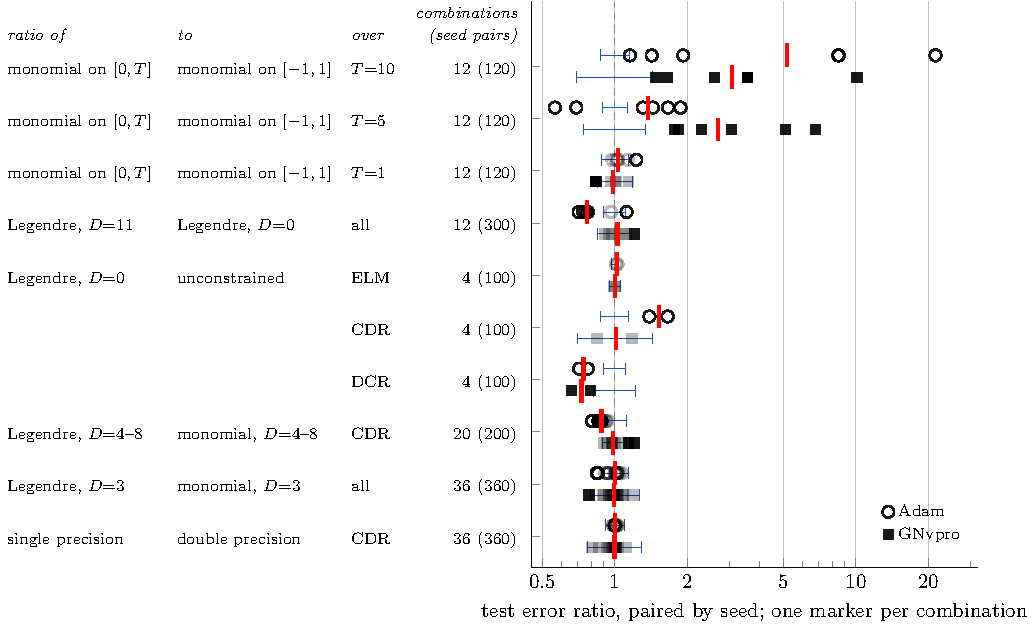
\includegraphics[width=\textwidth]{figures/effect_ledger.pdf}
    \caption{Paired test-error ratios for the ResNet and Hamiltonian experiments of
    Section~\ref{sect:ResNet_results}, which are trained by differentiating the discrete scheme.
    Every row compares two settings that differ in one respect, both named at the left, and the
    first of them is in the numerator, so a ratio below one means that setting has the lower test
    error. Every marker is one combination of dataset, architecture, optimizer and terminal time,
    drawn at the geometric mean over seeds of its per-seed ratio. Open circles are Adam and filled squares
    GNvpro, each with its median in red, since the two optimizers disagree in sign on the degree
    axis. The blue interval spans one seed-to-seed geometric standard deviation either side of
    parity, and a marker inside it is drawn pale, meaning the setting moves test error less than
    rerunning the same configuration with another seed. The last column gives the combinations in
    the row and the seed pairs behind them. Ten seeds per configuration, forty for GNvpro on the
    degree axis at $T=1$.}\label{fig:effect_ledger}
\end{figure}

\begin{figure}[!h]
    \centering
    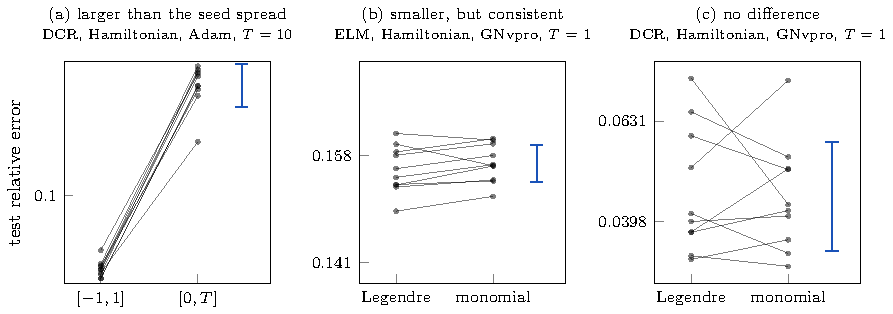
\includegraphics[width=\textwidth]{figures/paired_panels.pdf}
    \caption{Individual runs behind three comparisons in the ResNet and Hamiltonian experiments,
    with one line per seed joining the two runs that share it, so the slope of a line is that
    seed's paired ratio. The blue bar is one seed-to-seed geometric standard deviation of a single
    configuration, the spread that rerunning with another seed produces. Panel (a) shows a
    difference larger than that spread, the monomial basis on $[-1,1]$ against $[0,T]$ at $T=10$,
    for the DCR Hamiltonian variant under Adam, where every seed moves the same way and the ratio is $0.05$ [$0.04$, $0.06$]. Panel (b) shows a
    difference that is consistent across seeds and smaller than the spread, Legendre against
    monomial at degree $3$ for the ELM Hamiltonian variant under GNvpro at $T=1$, where Legendre is lower on eight of ten seeds at $0.993$ [$0.984$, $1.002$], an
    interval that includes parity. Panel (c) shows no difference, the same comparison for the DCR Hamiltonian variant under GNvpro at $T=1$, at $1.03$
    [$0.84$, $1.25$] with the seeds split five and five.}\label{fig:paired_panels}
\end{figure}

\begin{figure}[!h]
    \centering
    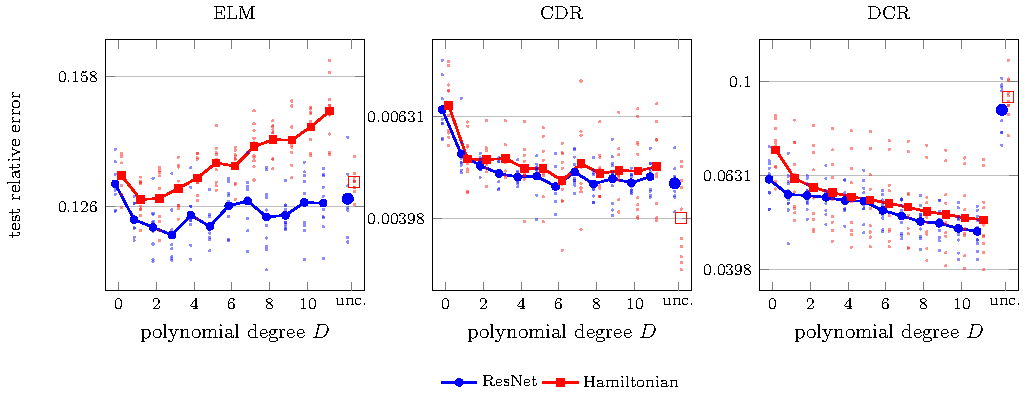
\includegraphics[width=0.86\textwidth]{figures/degree_lever.pdf}
    \caption{Test relative error of the ResNet and the Hamiltonian variant against polynomial
    degree $D$, at $T=1$ under Adam in the Legendre basis, with one panel per dataset. Dots are
    single seeds, offset left for the ResNet and right for the Hamiltonian variant, and each curve
    is the geometric mean over ten seeds, with the static-weight model at $D=0$. The markers at the
    right, labelled ``unc.'', are the unconstrained model, which spans the same function class as
    $D=11$ yet differs from it by nearly a factor of two on DCR. The two architectures differ by
    less than one seed-to-seed spread, so the figure does not draw them as though they were
    separated. Table~\ref{tab:degree_efficiency} gives the paired comparisons between degrees for
    both optimizers.}\label{fig:degree_lever}
\end{figure}

\begin{figure}[!h]
    \centering
    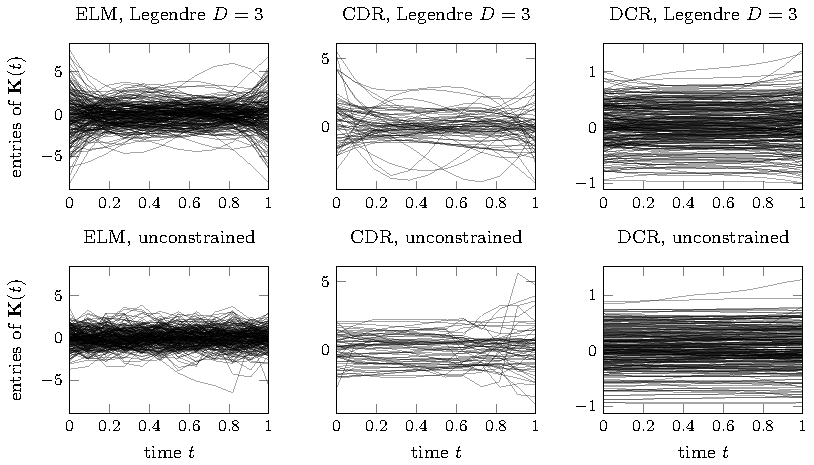
\includegraphics[width=0.86\textwidth]{figures/weight_trajectories.pdf}
    \caption{Entries of the learned weight matrix $\bfK(t)$ of the ResNet at its $N=12$ time
    points, at $T=1$ under Adam, for one seed, with the degree-$3$ Legendre model above and the
    unconstrained model below. The two panels of a column share one vertical scale. The weights
    vary in time on ELM and CDR and stay nearly constant on DCR. Over ten seeds the variation in
    time, $\|\bfK-\bar\bfK\|_F/\|\bfK\|_F$ with $\bar\bfK$ the time average, is $0.75$ to $0.84$ on
    ELM, $0.55$ to $0.69$ on CDR and $0.12$ to $0.17$ on DCR for the degree-$3$ model, and the
    roughness, the same ratio for the second difference in time, is $4.4$ to $7.0$ and $2.2$ to
    $4.2$ times larger for the unconstrained model on ELM and CDR and smaller on DCR on nine of ten
    seeds.}\label{fig:weight_trajectories}
\end{figure}

\begin{figure}[!h]
    \centering
    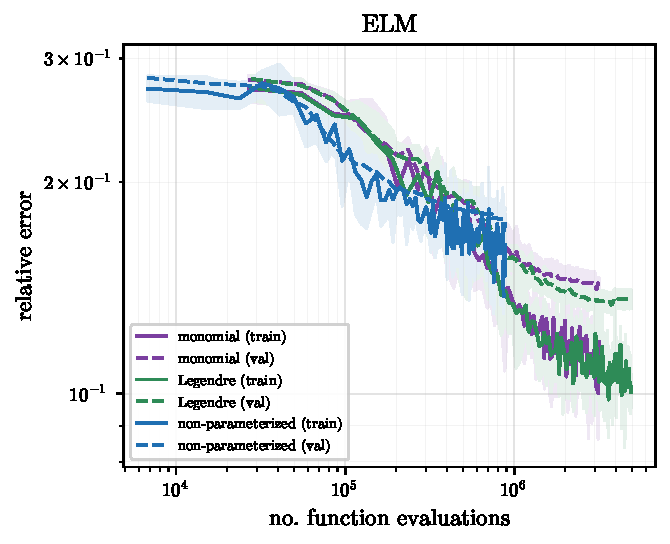
\includegraphics[width=0.33\textwidth]{figures/node_nfe_elm.pdf}\hfill
    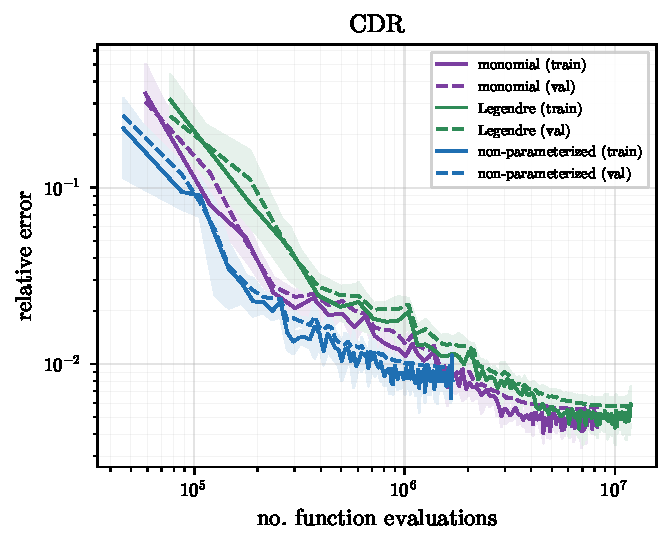
\includegraphics[width=0.33\textwidth]{figures/node_nfe_cdr.pdf}\hfill
    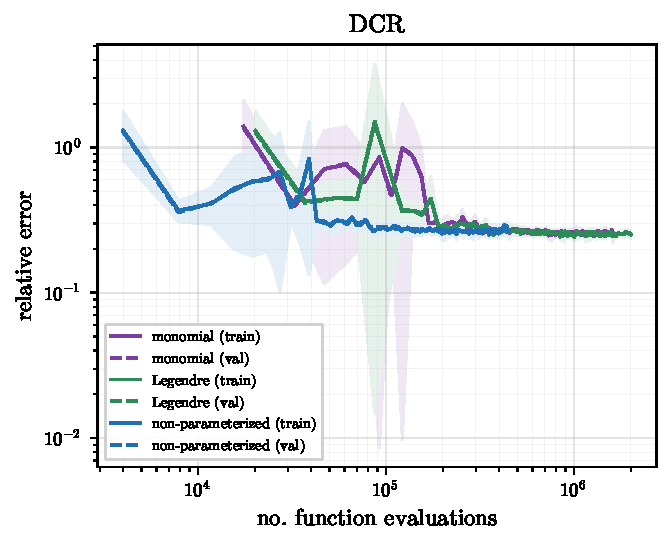
\includegraphics[width=0.33\textwidth]{figures/node_nfe_dcr.pdf}

    \caption{Training and validation error of the neural ODE, which is trained with the continuous
    adjoint, against the number of function evaluations at $T=1$, as the mean over five seeds, for
    the static model and for the degree-$3$ monomial and Legendre models. Parameterization lowers
    the error on ELM and CDR and not on DCR, and on all three it raises the number of function
    evaluations the adaptive solver needs, which Table~\ref{tab:meanstd} states as a
    number. Each seed's curve ends at its best validation iterate, so the last points of a curve
    average fewer than five seeds.}\label{fig:neuralODE_loss}
\end{figure}
 











\begin{appendices}

\section{Selected settings}\label{app:selection}

The regularization parameter was selected on validation error at $D=3$, $T=1$ and in the Legendre
basis, for both architectures and both optimizers. DCR decides the choice: at $\alpha=10^{-6}$ its
validation error is $1.8$ to $4.9$ times that at $10^{-10}$ and at $10^{-4}$ it is $4.7$ to $6.6$
times, whereas $10^{-8}$ and $10^{-10}$ differ by less than $1\%$ under Adam and are not separated
under GNvpro. On ELM and CDR a different value lowers the validation error, with a paired interval that excludes $1$, in four of the eight
combinations of dataset, architecture and optimizer, by $8\%$ and $2\%$ for the ELM Hamiltonian
variant at $\alpha=10^{-4}$ under Adam and GNvpro, by $1\%$ for the ELM ResNet at $10^{-5}$ under
GNvpro, and by $34\%$ for the CDR Hamiltonian variant at $10^{-8}$ under GNvpro. We use $\alpha=10^{-10}$ throughout so that every comparison shares one
regularization.

\section{The training budget}\label{app:budget}

On ELM the best validation iterate of Adam arrives at $64\%$ of the budget in the median, so most
ELM models are compared after their validation error has stopped improving. On DCR and CDR it
arrives at $98\%$ and $100\%$, with $75\%$ and $96\%$ of runs peaking in the final twentieth.
Because we did not observe convergence there, we re-ran $D=0$, $D=11$ and the unconstrained model
at five times the budget, $10{,}000$ epochs on DCR and $50{,}000$ on CDR, with five seeds. The
median best iterate still arrives at $99\%$ of the budget, and test error falls in all twelve
combinations of dataset, architecture and model, to between $0.54$ and $0.69$ times its value. The
comparisons between models change little: on DCR the ratio of the degree-$11$ model's test error to
the unconstrained model's, on the five seeds of the re-run, is $0.53$ [$0.44$, $0.64$] at the original budget and $0.60$ [$0.53$,
$0.68$] at five times the budget for the ResNet, and $0.58$ and $0.59$ for the Hamiltonian variant,
while on CDR both intervals include $1$ at either budget. GNvpro's best iterate arrives at a median
of $11$ iterations on ELM and DCR and $17$ on CDR.

\section{Test error by configuration}\label{app:table2}

\begin{table}[!htb]
\caption{Test relative error~\eqref{eq:relerr} by architecture, optimizer, and terminal time ($T$) for ELM, DCR, and CDR, using a third-degree Legendre or monomial basis unless labeled ``none'' (the non-parameterized baseline, which spans the same function class as degree $N-1$). The number of time steps is fixed at $N=12$, so increasing $T$ increases the step size rather than the depth. Params is the dynamics-only $\bftheta_{\rm NODE}$ count, excluding the dataset-specific readout $\bfK_{\rm out},\bfb_{\rm out}$; it varies across datasets because the channel width does. Each cell is the geometric mean over ten seeds, as a mantissa against the power of ten named with each dataset, with the geometric standard deviation as a multiplicative factor in parentheses, and each block reports the error of the trivial predictor that returns the training mean.}\label{tab:ComprehensiveLegendre}
    \centering
    % body generated by matlab/analysis/makeTableC1.m; regenerate with `make tables`
    \setlength{\tabcolsep}{4pt}
    % generated 2026-10-06 06:19:44 from commit 259ce29 by MATLAB R2026a on MacBook-Pro
% source: results/runs.csv   sweep: 2026-10-02-paper
% regenerate with: makeTableC1('2026-10-02-paper')
% metric: aggregate relative error ||Pred-C||_F/||C||_F on the test set
% cells are the geometric mean over 10 seeds (geometric standard deviation as a factor),
% printed as a two-digit mantissa against the power of ten named with each dataset
\begin{tabular}{llcccccc}
\toprule
& & & & \multicolumn{2}{c}{ResNet} & \multicolumn{2}{c}{Hamiltonian} \\
\cmidrule(lr){5-6} \cmidrule(lr){7-8}
Dataset & Parameterization & Params & $T$ & Adam & GNvpro & Adam & GNvpro \\
\midrule
\cmidrule(lr){2-8}
ELM & \multirow{3}{*}{Legendre ($D=3$)} & \multirow{3}{*}{960} & $T=1$ & $1.2\,(1.05)$ & $1.6\,(1.08)$ & $1.3\,(1.04)$ & $1.6\,(1.03)$ \\  % n=[10 10 10 10] seeds
$(\times 10^{-1})$ & &  & $T=5$ & $1.3\,(1.08)$ & $2.0\,(1.06)$ & $1.3\,(1.06)$ & $1.8\,(1.08)$ \\  % n=[10 10 10 10] seeds
 & &  & $T=10$ & $1.9\,(1.32)$ & $2.6\,(1.06)$ & $2.7\,(1.12)$ & $2.8\,(1.06)$ \\  % n=[10 10 10 10] seeds
\cmidrule(lr){2-8}
 & \multirow{3}{*}{monomial ($D=3$)} & \multirow{3}{*}{960} & $T=1$ & $1.2\,(1.04)$ & $1.6\,(1.08)$ & $1.3\,(1.04)$ & $1.6\,(1.02)$ \\  % n=[10 10 10 10] seeds
 & &  & $T=5$ & $1.2\,(1.05)$ & $2.0\,(1.07)$ & $1.3\,(1.04)$ & $1.7\,(1.08)$ \\  % n=[10 10 10 10] seeds
 & &  & $T=10$ & $1.8\,(1.37)$ & $2.6\,(1.07)$ & $2.6\,(1.11)$ & $2.7\,(1.07)$ \\  % n=[10 10 10 10] seeds
\cmidrule(lr){2-8}
 & \multirow{3}{*}{none} & \multirow{3}{*}{2880} & $T=1$ & $1.3\,(1.05)$ & $1.7\,(1.05)$ & $1.3\,(1.02)$ & $1.6\,(1.07)$ \\  % n=[10 10 10 10] seeds
 & &  & $T=5$ & $1.7\,(1.17)$ & $2.1\,(1.05)$ & $1.3\,(1.07)$ & $1.9\,(1.13)$ \\  % n=[10 10 10 10] seeds
 & &  & $T=10$ & $2.6\,(1.24)$ & $2.6\,(1.11)$ & $3.0\,(1.06)$ & $3.0\,(1.04)$ \\  % n=[10 10 10 10] seeds
\cmidrule(lr){2-8}
& \emph{mean predictor} & & & \multicolumn{4}{c}{5.3} \\
\midrule
\cmidrule(lr){2-8}
DCR & \multirow{3}{*}{Legendre ($D=3$)} & \multirow{3}{*}{1088} & $T=1$ & $5.7\,(1.09)$ & $4.4\,(1.30)$ & $5.8\,(1.20)$ & $4.6\,(1.34)$ \\  % n=[10 10 10 10] seeds
$(\times 10^{-2})$ & &  & $T=5$ & $3.3\,(1.05)$ & $2.5\,(1.27)$ & $3.0\,(1.12)$ & $2.5\,(1.28)$ \\  % n=[10 10 10 10] seeds
 & &  & $T=10$ & $3.0\,(1.10)$ & $3.0\,(1.26)$ & $2.7\,(1.21)$ & $3.9\,(1.68)$ \\  % n=[10 10 10 10] seeds
\cmidrule(lr){2-8}
 & \multirow{3}{*}{monomial ($D=3$)} & \multirow{3}{*}{1088} & $T=1$ & $5.5\,(1.14)$ & $4.6\,(1.41)$ & $5.7\,(1.19)$ & $4.5\,(1.29)$ \\  % n=[10 10 10 10] seeds
 & &  & $T=5$ & $3.3\,(1.16)$ & $2.3\,(1.25)$ & $3.2\,(1.12)$ & $3.2\,(1.63)$ \\  % n=[10 10 10 10] seeds
 & &  & $T=10$ & $2.9\,(1.16)$ & $3.2\,(1.23)$ & $2.9\,(1.15)$ & $4.3\,(1.66)$ \\  % n=[10 10 10 10] seeds
\cmidrule(lr){2-8}
 & \multirow{3}{*}{none} & \multirow{3}{*}{3264} & $T=1$ & $8.7\,(1.12)$ & $5.7\,(1.19)$ & $9.3\,(1.11)$ & $5.8\,(1.20)$ \\  % n=[10 10 10 10] seeds
 & &  & $T=5$ & $4.4\,(1.14)$ & $3.0\,(1.55)$ & $3.4\,(1.14)$ & $1.9\,(1.51)$ \\  % n=[10 10 10 10] seeds
 & &  & $T=10$ & $3.5\,(1.12)$ & $3.5\,(1.47)$ & $3.5\,(1.31)$ & $3.3\,(1.73)$ \\  % n=[10 10 10 10] seeds
\cmidrule(lr){2-8}
& \emph{mean predictor} & & & \multicolumn{4}{c}{100} \\
\midrule
\cmidrule(lr){2-8}
CDR & \multirow{3}{*}{Legendre ($D=3$)} & \multirow{3}{*}{288} & $T=1$ & $4.9\,(1.05)$ & $12\,(1.19)$ & $5.2\,(1.08)$ & $16\,(1.52)$ \\  % n=[10 10 10 10] seeds
$(\times 10^{-3})$ & &  & $T=5$ & $5.0\,(1.09)$ & $11\,(1.61)$ & $4.9\,(1.10)$ & $15\,(1.22)$ \\  % n=[10 10 10 10] seeds
 & &  & $T=10$ & $5.0\,(1.12)$ & $24\,(2.42)$ & $6.4\,(1.15)$ & $59\,(3.60)$ \\  % n=[10 10 10 10] seeds
\cmidrule(lr){2-8}
 & \multirow{3}{*}{monomial ($D=3$)} & \multirow{3}{*}{288} & $T=1$ & $5.3\,(1.14)$ & $11\,(1.09)$ & $5.6\,(1.22)$ & $17\,(1.60)$ \\  % n=[10 10 10 10] seeds
 & &  & $T=5$ & $6.0\,(1.16)$ & $11\,(1.62)$ & $5.8\,(1.15)$ & $17\,(1.45)$ \\  % n=[10 10 10 10] seeds
 & &  & $T=10$ & $4.9\,(1.13)$ & $20\,(2.60)$ & $6.8\,(1.32)$ & $54\,(3.45)$ \\  % n=[10 10 10 10] seeds
\cmidrule(lr){2-8}
 & \multirow{3}{*}{none} & \multirow{3}{*}{864} & $T=1$ & $4.7\,(1.08)$ & $12\,(1.17)$ & $4.0\,(1.21)$ & $15\,(1.49)$ \\  % n=[10 10 10 10] seeds
 & &  & $T=5$ & $4.4\,(1.11)$ & $10\,(1.59)$ & $4.2\,(1.12)$ & $12\,(1.08)$ \\  % n=[10 10 10 10] seeds
 & &  & $T=10$ & $4.8\,(1.22)$ & $29\,(2.81)$ & $4.8\,(1.15)$ & $57\,(3.91)$ \\  % n=[10 10 10 10] seeds
\cmidrule(lr){2-8}
& \emph{mean predictor} & & & \multicolumn{4}{c}{206} \\
\bottomrule
\end{tabular}

\end{table}

\end{appendices}

\section*{Statements and declarations}

\begin{itemize}
    \item Funding: L.R.'s and H.R.'s work was partially supported by the US National Science Foundation under grant DMS 2038118. 
    This work is partially supported by Sandia National Laboratories' Laboratory Directed Research and Development (LDRD) program. 
KS also acknowledges support by the U.S. Department of Energy, Office of Science, Office of Advanced Scientific Computing Research (ASCR), 
Scientific Discovery through Advanced Computing (SciDAC) program, under the FASTMath Institute. 
    \item Conflict of interest: The authors declare that they have no known competing financial interests or personal relationships that could have appeared to influence the work reported in this paper.
    \item Author contributions: H.R. wrote the main manuscript text, prepared figures and tables, and performed experiments and analysis of results. L.R. provided supervision, formed methodology,  and reviewed and edited the main manuscript text. K.S. conceptualized the project, formed methodology, and provided funding and technical resources.
    \item Use of AI tools: The authors used AI tools as a writing aid, as a coding assistant, and for literature search. The authors checked all text, code, and references produced with these tools and take full responsibility for the content of this paper.
    \item Data availability: The ELM and CDR datasets are included in the repository below.
    %
    The DCR dataset is too large to distribute with the code and is archived
    at~\href{https://doi.org/10.5281/zenodo.21537966}{this Zenodo record}; \texttt{data/setupDCR.m}
    fetches it.
    %
    All three are used through a single fixed index permutation, exported once by
    \texttt{exportSplits.m} and shared by both halves of the code, so the MATLAB and PyTorch
    experiments train and test on bit-identical samples rather than on nominally identical seeds.
    %
    \item Code availability: The manuscript and the code that produces every table and figure in it
    live in one repository, \url{https://github.com/EmoryMLIP/2026-WeightParameterizationNODE}.
    %
    Each experiment writes a per-run record carrying the commit that produced it; those records are
    collected into a ledger, and the tables are generated from the ledger rather than transcribed,
    so every number in Section~\ref{sect:results} can be traced to the runs behind it and rebuilt
    without retraining.
    %
    The repository states which sweep backs which table, and which sweeps have been superseded and
    why; superseded results are retained rather than deleted.
    %
    The regularization strength, the readout initialization, and the optimizer settings of the
    neural ODE experiments are selected on validation error, and each selection is recorded with
    the sweep that determined it.
    %
    The ResNet experiments use a fork of the MATLAB Meganet library~\cite{HaberRuthotto2017}
    reduced to the components this manuscript needs; the four local modifications to it are marked
    in place. The neural ODE experiments use PyTorch with \texttt{torchdiffeq}.
    %
    A test suite covering the basis construction, the Gram matrix, the continuous adjoint against
    backpropagation, and a Taylor convergence rate must pass before any sweep is run.

    \item Ethics approval: not applicable.
    \item Consent to participate: not applicable.
    \item Consent for publication: not applicable. 
    \item This article has been co-authored by employees of National Technology \& Engineering Solutions of Sandia, LLC under Contract No. DE-NA0003525 
with the U.S. Department of Energy (DOE). The employees co-own right, title and interest in and to the article and are responsible for its contents. 
The United States Government retains and the publisher, by accepting the article for publication, acknowledges that the United States Government 
retains a non-exclusive, paid-up, irrevocable, world-wide license to publish or reproduce the published form of this article or allow others to do so, 
for United States Government purposes. The DOE will provide public access to these results of federally sponsored research in 
accordance with the \href{https://www.energy.gov/downloads/doe-public-access-plan}{DOE Public Access Plan}. 
\end{itemize}





\newpage
\bibliography{main}

\end{document}